\begin{center}
\textit{by A. Benaglia, M. Bengala, O. Bondu, L. Borgonovi, S. Braibant, L. Cadamuro, A. Carvalho, C. Delaere, M. Delcourt, N. de Filippis, E. Fontanesi, M. Gallinaro, M. Gouzevitch, J. R. Komaragiri, D. Majumder, K. Mazumdar, F. Monti, G. Ortona, L. Panwar, N. Sahoo, R. Santo, G. Strong, M. Vidal, S. Wertz}
\end{center}

The work described in this section studies the prospects for \HH production at the HL-LHC with the CMS experiment.
The five decay channels \bbbb, \bbtt, \bbWW ($\PW\PW\to\ell\nu\ell'\nu'$ with $\ell,\ell' = \Pe,\Pgm$), \bbgg, and \bbZZ ($\PZ\PZ\to\ell\ell\ell'\ell'$ with $\ell,\ell' = \Pe,\Pgm$) are explored.
The corresponding branching fractions and the total number of \HH events expected to be produced at the HL-LHC assuming $\sqrt{s} = 14\TeV$ and an integrated luminosity of $3000\fbi$ are reported in Table~\ref{sec3:CMSHH:tab:br_nevent}.

A short description of the analysis strategy and of the results is given here, and further details can be found in Ref.~\cite{CMS-PAS-FTR-18-019}.

\begin{table}[h]
  \begin{center}
    \caption{Branching fraction of the five decay channels considered in the CMS \HH prospects, and corresponding number of events produced at the end of HL-LHC operations assuming $\sqrt{s} = 14\TeV$ and an integrated luminosity of $3000\fbi$. The symbol $\ell$ denotes either a muon or an electron. In the \bbWW decay channel, $\ell$ from the intermediate production of a $\tau$ lepton are also considered in the branching fraction.}
    \label{sec3:CMSHH:tab:br_nevent}
    \begin{tabular}{l  ccccc}
        \hline
        Channel            & $\bbbb$ & $\bbtt$ & $\bbWW(\ell\nu\ell\nu)$ & $\bbgg$ & $\bbZZ(\ell\ell\ell\ell)$ \\
        $\mathcal{B}$ [\%] & 33.9    & 7.3     & 1.7                    & 0.26    & 0.015\\
        Number of events   & 37000   & 8000    & 1830                   & 290     & 17\\
        \hline      
    \end{tabular}
  \end{center}
\end{table}

A parametric simulation based on the \delphes~\cite{deFavereau:2013fsa} software is used to model the CMS detector response in the HL-LHC conditions.
The \delphes simulation accounts for the effects of multiple  hadron interactions (``pileup'') by overlaying simulated minimum-bias events with on average 200 interactions per bunch crossing.
The performance of reconstruction and identification algorithms for electrons, muons, tau decays to hadrons (\tauh) and a neutrino, photons, jets (including the identification of those containing heavy flavour particles), and the missing transverse momentum vector \ptvecmiss is parametrised based on the  results obtained with a full simulation of the CMS detector and dedicated reconstruction algorithms.


\paragraph{The $\HH\to\bbbb$ channel}

While characterised by the largest branching fraction among the $\HH$ final states, the \bbbb decay channel suffers from a large contamination from the multi-jet background that makes it experimentally challenging.
Two complementary strategies are explored here to identify the signal contribution.
For those events where the four jets from the $\HH\to\bbbb$ decay can all be reconstructed separately, also referred to as the ``resolved'' topology, the usage of multivariate methods is explored to efficiently identify the signal contribution in the overwhelming background.
In cases where the invariant mass of the $\HH$ system, $m_{\HH}$, is large, the high Lorentz boost of both Higgs bosons may results in a so-called ``boosted'' event topology where the two jets from a $\Hbb$ decay overlap and are reconstructed as a single, large-area jet.
Resolved topologies correspond to the large majority of SM \HH events, giving the largest sensitivity on this signal.
Boosted topologies help to suppress the multi-jet background and provide sensitivity to BSM scenarios where the differential \HH production cross section is enhanced at high $m_{\HH}$ by the presence of $\Pg\Pg\HH$ and $\PQt\PQt\HH$ effective contact interactions.

In the resolved topology, events are pre-selected by requiring four jets with $\pt > 45~\GeV$ and $|\eta| <$ 3.5 that satisfy the medium b-tagging working point, corresponding to a b jet identification efficiency of approximately 70\% for a light  flavour and gluon jet mis-identification rate of  1\%.
Triggers are assumed to be fully efficient in the phase space defined by this selection.
In scenarios where the minimal jet trigger \pt threshold is increased the loss in sensitivity to the SM signal amounts to approximately 10\% and 25\% for a 10 and 30\GeV increase, respectively.

The four selected b tagged jets are combined into the two Higgs boson candidates $\PH_1$ and $\PH_2$, choosing the pairs of jets with the minimal invariant mass difference.
The invariant mass of the two Higgs candidates is required to satisfy the relation:
\begin{equation}
\sqrt{ \left( \text{m}_{\PH_1} - 120\GeV\right)^2 + \left( \text{m}_{\PH_2} - 120\GeV\right)^2 } < 40\GeV
\end{equation}
i.e. a circular selection where the centre and radius are chosen based on the expected response and resolution of the CMS detector, accounting for the energy loss from undetected neutrinos from B hadron decays.

Because of the very large QCD multi-jet background, a multivariate discriminant, in the form of a boosted decision tree, is trained to identify the \HH signal contribution and used as the discriminant variable.
Other background processes considered are \ttbar and single Higgs boson production.
The output of the BDT discriminant is shown in Fig.~\ref{sec3:CMSHH:fig:bbbb_BDT}.

\begin{figure}[!htb]
\centering 
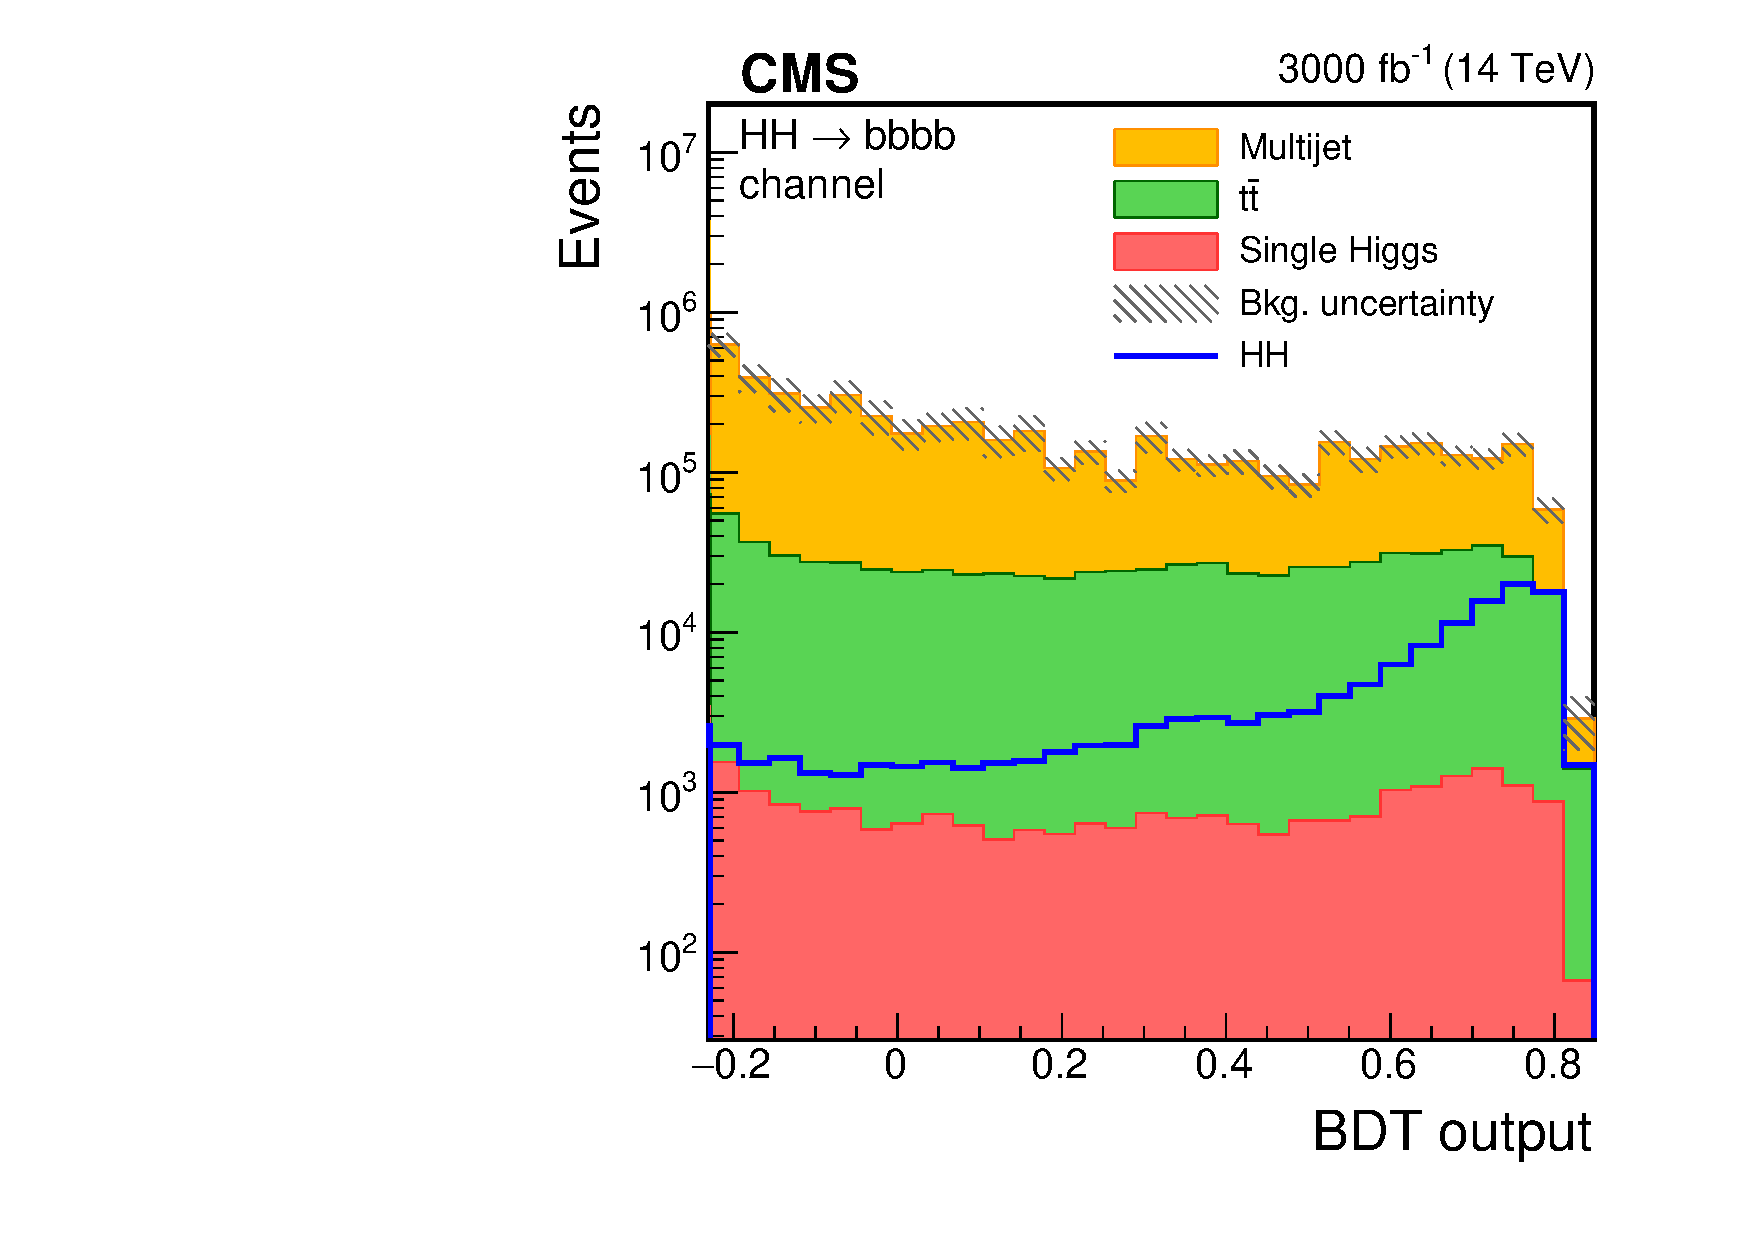
\includegraphics[width=0.5\textwidth]{\main/section3/plots/CMS/plot_BDTG_6_masscut_finalsel_log.pdf}
\caption{BDT output distribution for the signal and background processes considered in the \bbbb resolved search.} 
\label{sec3:CMSHH:fig:bbbb_BDT} 
\end{figure}

The boosted topology offers a good handle to investigate effective Higgs boson contact interactions predicted in BSM scenarios that enhance the \HH production cross section at high $m_{\HH}$ values.
For that reason, the prospects in this channels focus on anomalous couplings and make use of the shape benchmarks signals described in Ref.~\cite{Carvalho2016}.
Large radius jets, clustered with the anti-$k_\text{T}$ algorithm with a cone radius of 0.8 (AK8 jets), are used to identify the  overlapping b jets.
The event is required to contain at least two AK8 jets with $\pt > 300\GeV$ and $|\eta| < 3$.
The two highest $\pt$ jets are chosen in case multiple candidates satisfy such requirements.
The soft drop~\cite{Dasgupta:2013ihk,Larkoski:2014wba} jet grooming algorithm is used to remove soft and collinear components of the jet and retain the two sub-jets associated with the showering and hadronisation of the two b quarks from the $\PH\to\PQb\PAQb$ decay.
A selection is applied on the N-sub-jettiness variable~\cite{Thaler:2011gf} to reduce the background contamination, mostly represented by di-jet production from QCD interactions.
Algorithms for the b jet identification are applied on the sub-jets with a working point corresponding to an efficiency of about 49\% for genuine b jets for a mis-identification rate of light flavour and gluon jets of about 1\%.
Events are divided in two categories if they contain exactly three (3b category) or exactly four (4b category) b-tagged sub-jets.

The invariant mass of the two selected AK8 , $M_{JJ}$, is used to look for the presence of a signal. Its distribution is shown in Fig.~\ref{sec3:CMSHH:fig:bbbb_boosted} for the two event categories.

\begin{figure}[!htb]
\centering 
    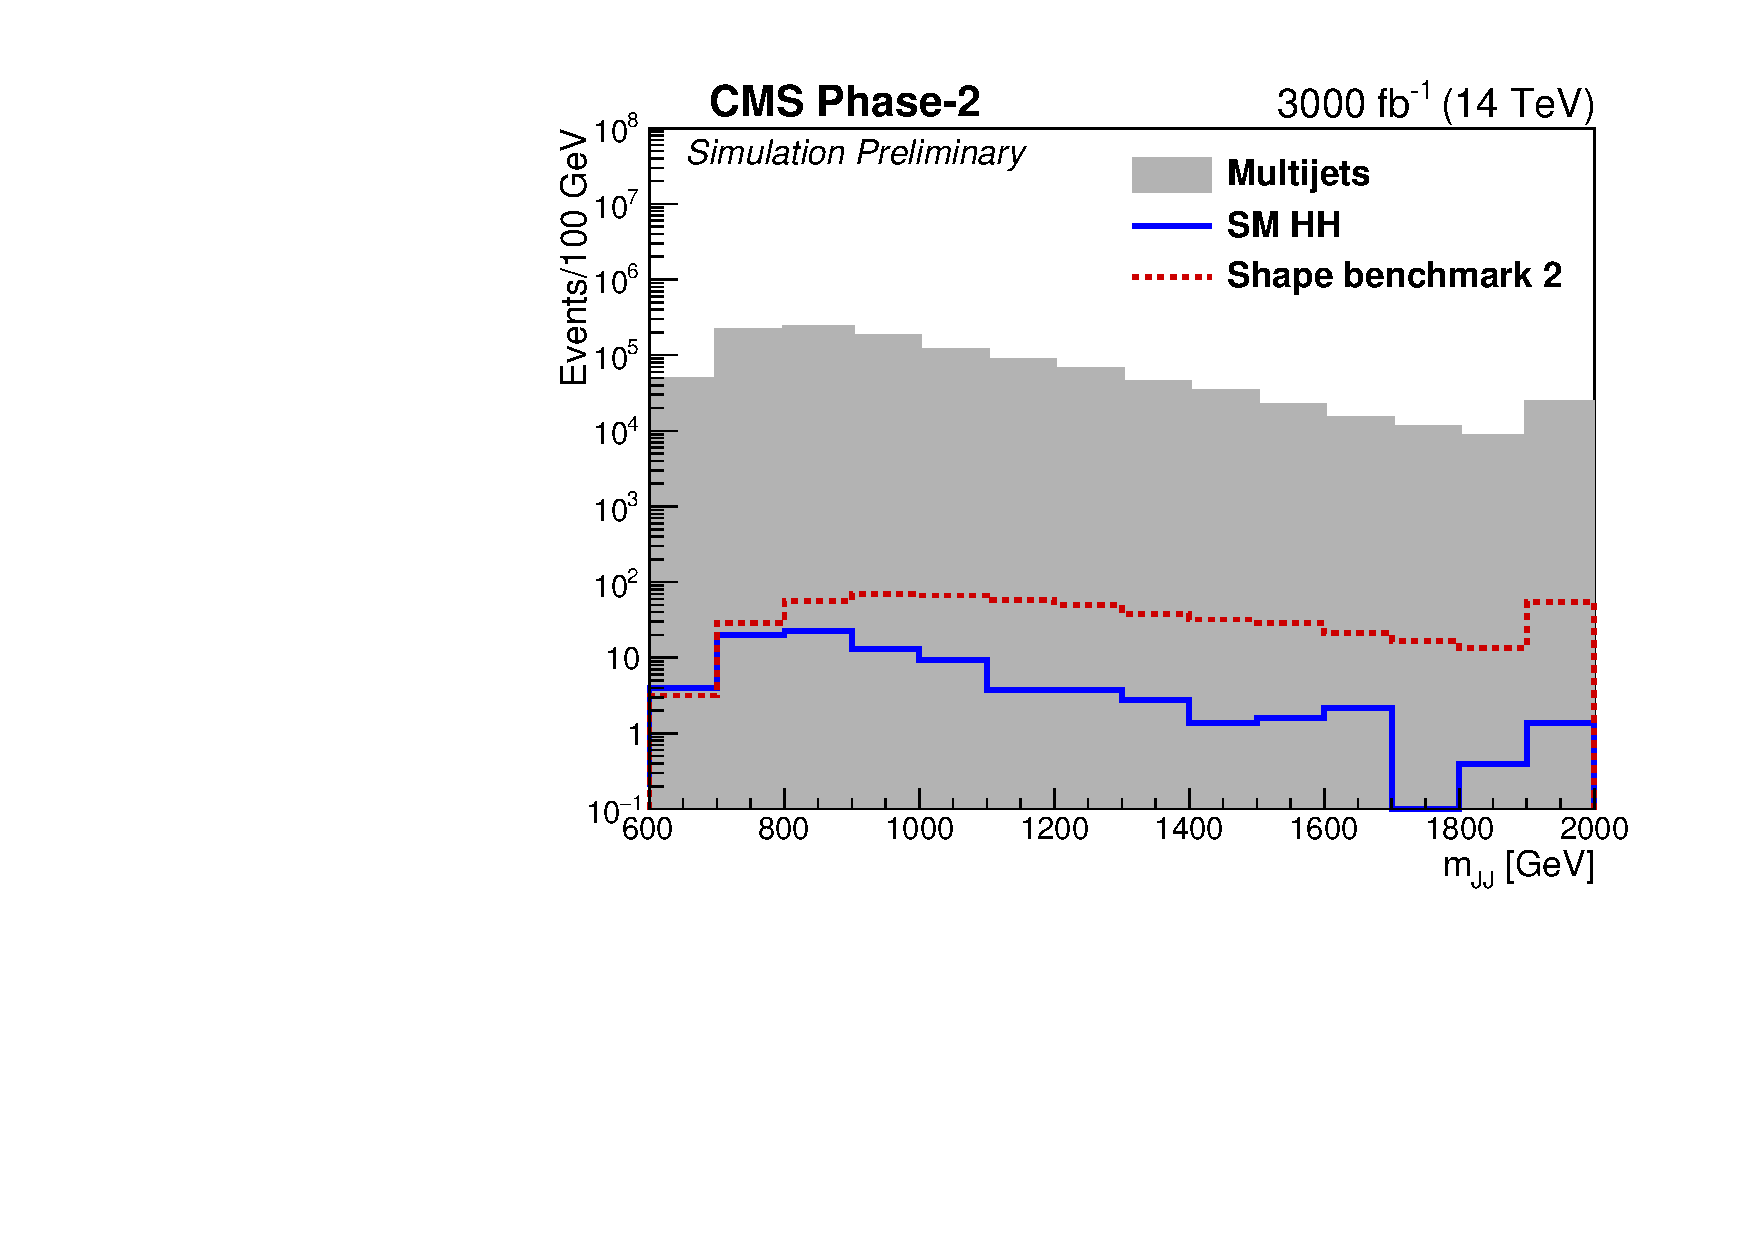
\includegraphics[width=0.495\textwidth]{\main/section3/plots/CMS/c_compare_h_mjj_3b_200_Logy1.pdf}
    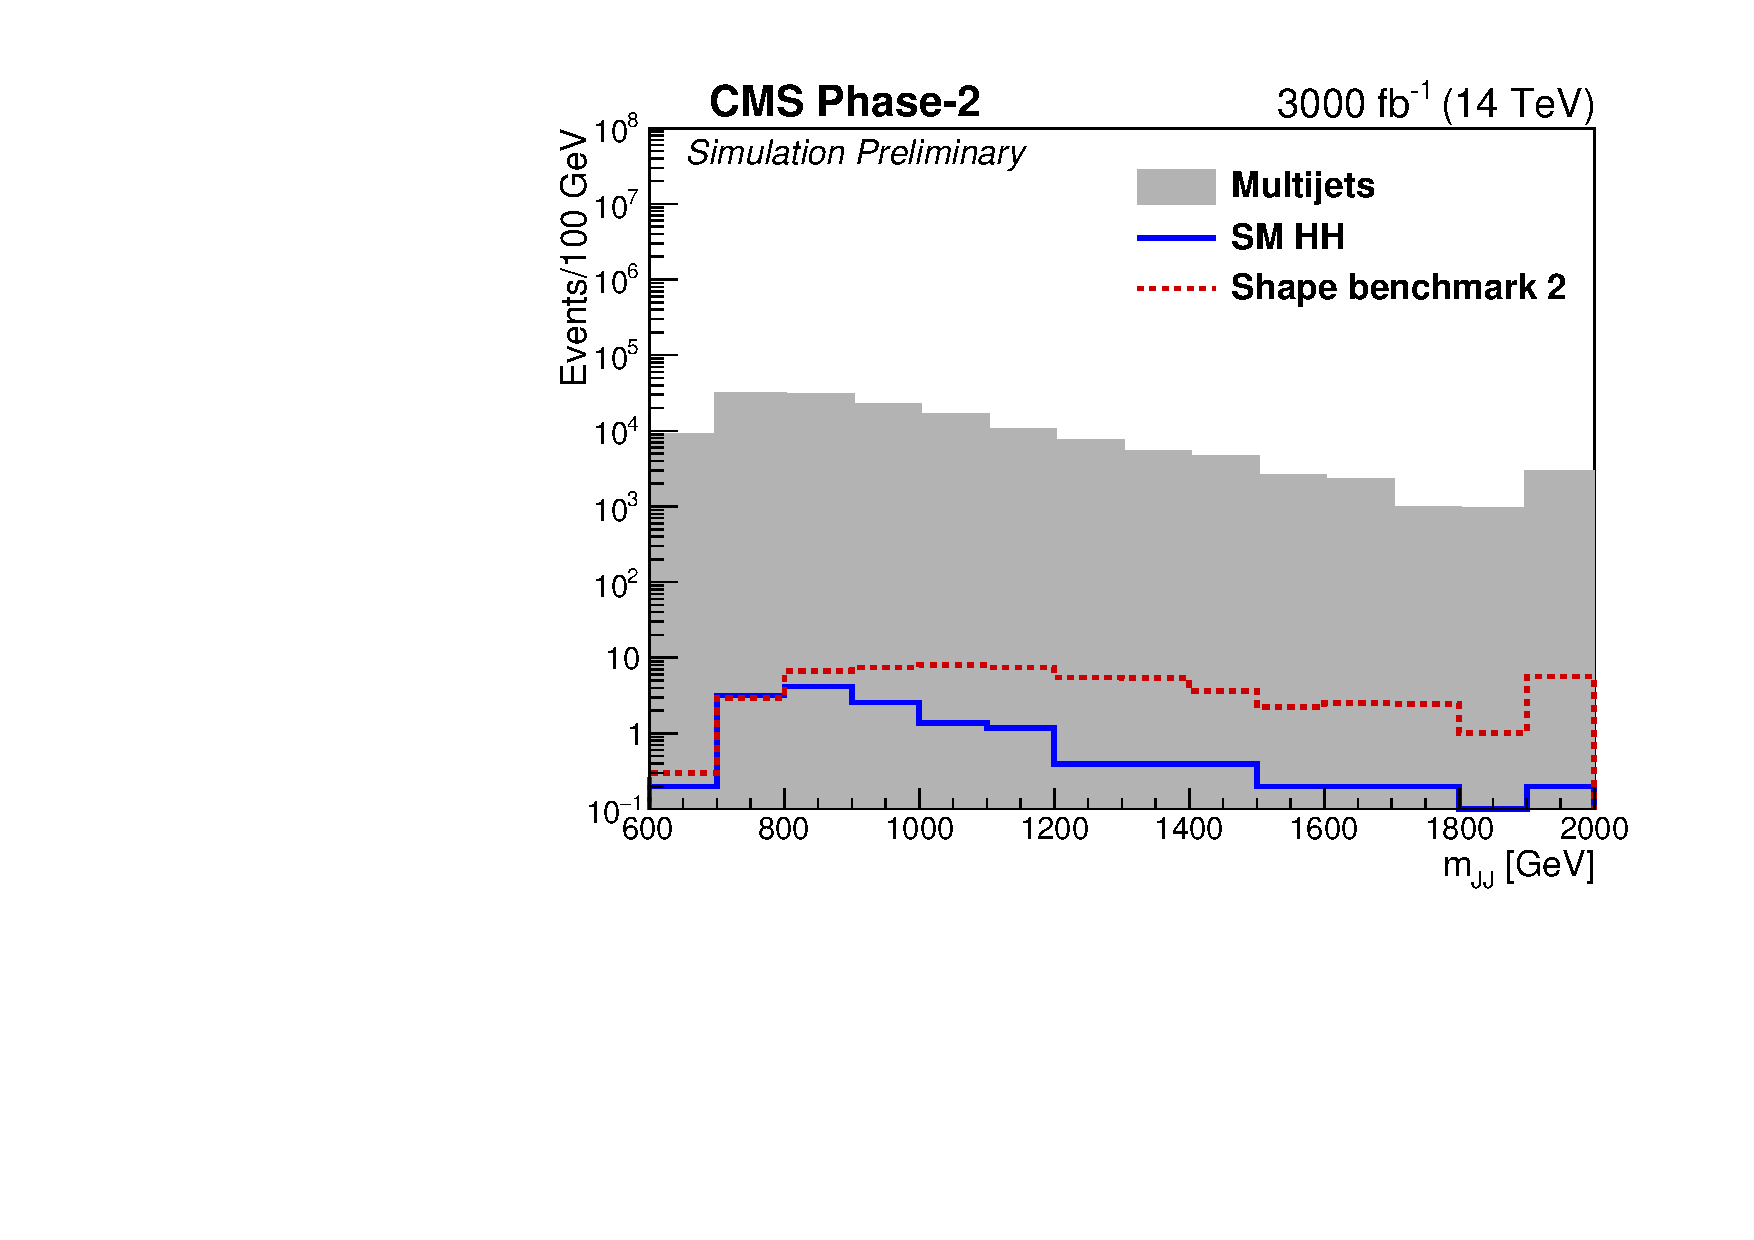
\includegraphics[width=0.495\textwidth]{\main/section3/plots/CMS/c_compare_h_mjj_4b_200_Logy1.pdf}
\caption{Invariant mass of the two selected AK8 jets in the boosted \bbbb \HH search for the multi-jet background and the SM (blue) and shape benchmark 2 (red) signals.
    The distributions on the left are for the $3\PQb$ and those on the right are for the $4\PQb$ sub-jet $\PQb$-tagged categories.
    Both signals are normalised to the SM $\PH\PH$ production cross section for visualisation.} 
\label{sec3:CMSHH:fig:bbbb_boosted} 
\end{figure}



\paragraph{The $HH \rightarrow \bbtt$ channel}

The $\bbtt$ decay channel is experimentally favourable thanks to its sizeable branching fraction of 7.3\% and the moderate background contamination.
Out of the six possible decay channels of the $\tau\tau$ system, the $\mu\tauh$, $\Pe\tauh$, and $\tauh\tauh$ final states are considered here, corresponding together to about 88\% of the total branching ratio.
Events in the three channels are selected requiring the presence of a \tauh candidate in association to an isolated muon, electron, or another \tauh\ depending on the final state considered.
Events in all the three categories above are then required to contain at least two b-tagged jets with $\pt > 30\GeV$ and $|\eta| < 2.4$. 

The main backgrounds are \ttbar and Drell-Yan production of $\tau$ pairs.
Their separation is experimentally challenging because of the incomplete reconstruction of the event due to the presence of neutrinos from $\tau$ decays that escape detection.

A multivariate analysis method is thus used to identify the signal contribution and separate if from the large background.
The usage of state-of-the-art machine learning techniques is studied in this work.
The discriminant consists of a pair of ensembles of ten fully connected deep neural networks (DNN), each with three hidden layers of 100 neurons, trained to separate the \HH signal from the background processes using a wide set of kinematic variables, a few of which are shown for illustration in Fig.~\ref{sec3:CMSHH:fig:bbttinputs}.
Each network is trained using events from all three $\tau\tau$ decay channels, and advanced optimisation techniques are explored and applied to maximise the expected sensitivity.

\begin{figure}[!htb]
\centering 
    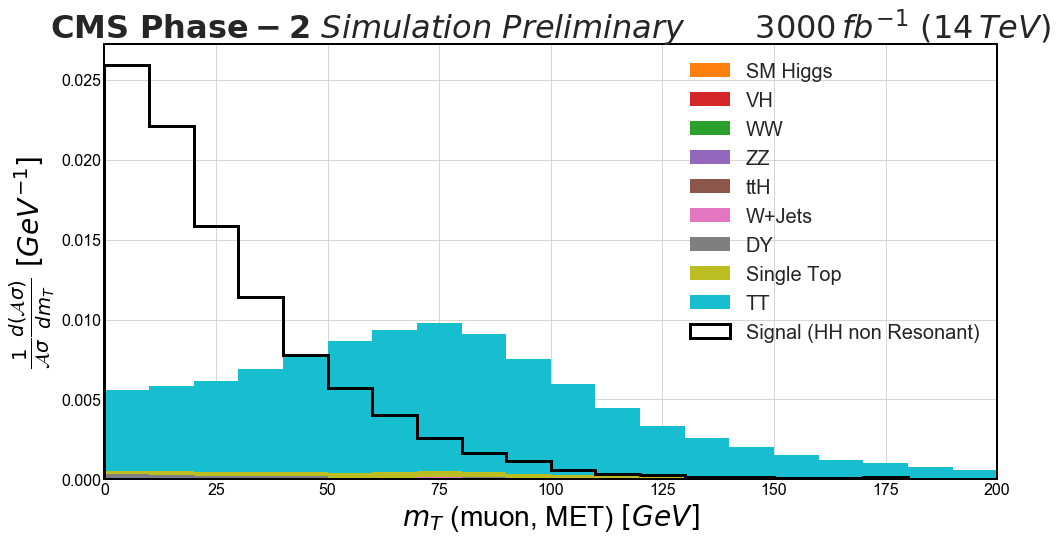
\includegraphics[width=0.495\textwidth]{\main/section3/plots/CMS/figure5a.png}
    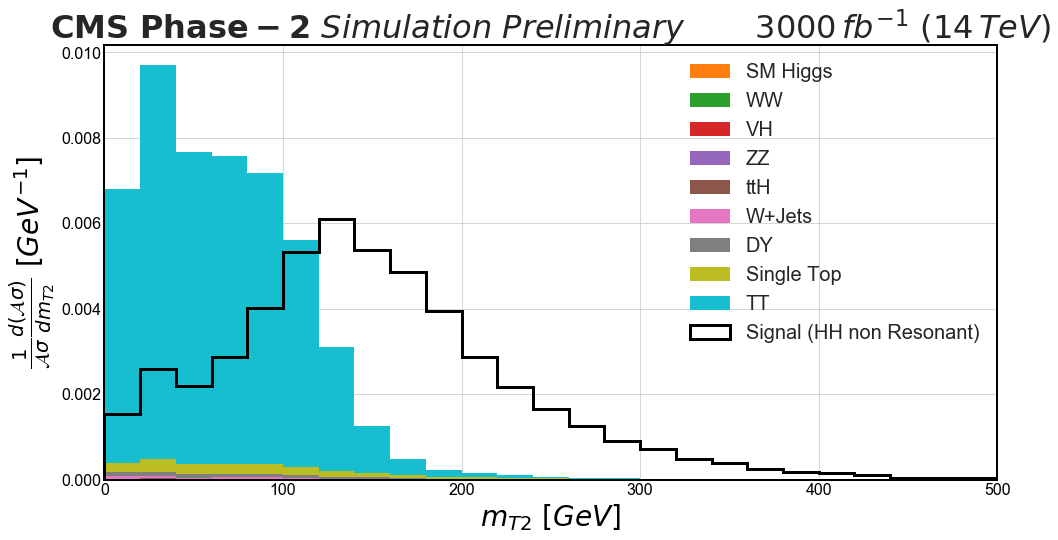
\includegraphics[width=0.495\textwidth]{\main/section3/plots/CMS/figure5e.png}\\
    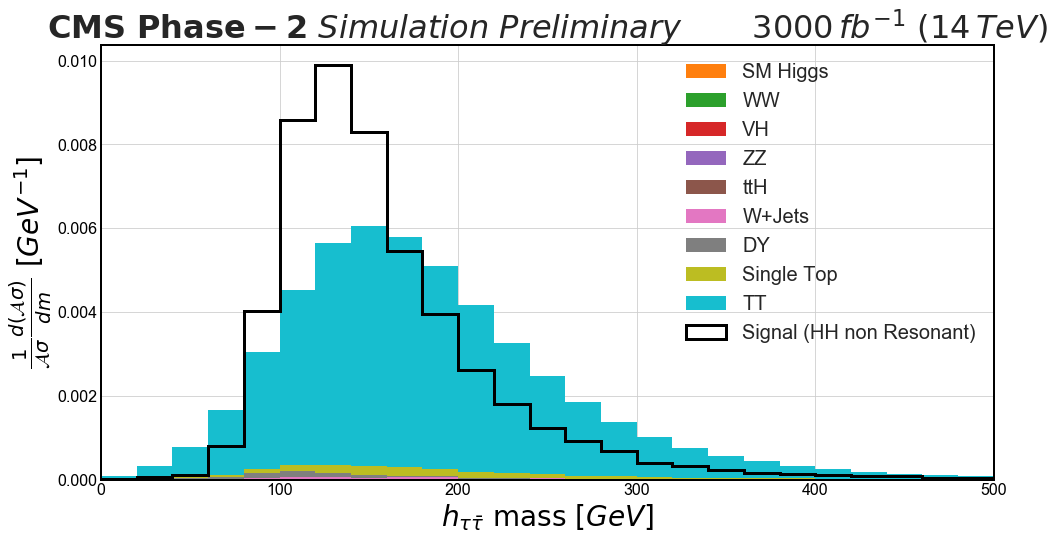
\includegraphics[width=0.495\textwidth]{\main/section3/plots/CMS/figure5c.png}
    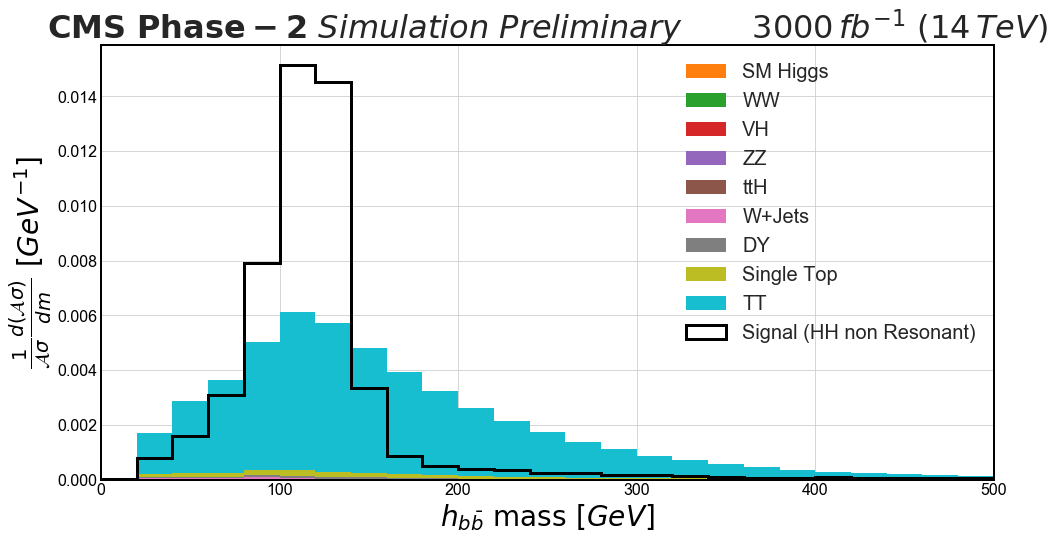
\includegraphics[width=0.495\textwidth]{\main/section3/plots/CMS/figure5d.png}\\    
\caption{Example distributions for some of the discriminant variables used as input of the \bbtt deep neural network for the $\mu\tauh$ final-state: muon transverse mass (top left), system transverse mass $m_\text{T2}$ (top right), and invariant mass of the $\tau\tau$ (bottom left) and bb (bottom right) systems.} 
\label{sec3:CMSHH:fig:bbttinputs} 
\end{figure}


\paragraph{The $HH \rightarrow b\bar{b}\gamma\gamma$ channel}

Despite its low branching fraction, the \bbgg decay channel is one of the most sensitive to \HH production.
It benefits of an excellent di-photon invariant mass ($m_{\gamma\gamma}$) resolution and on the possibility to fully reconstruct all final state objects.
The analysis strategy combines these two aspects and uses a multivariate kinematic discriminant to suppress the background contributions, and the $m_{\gamma\gamma}$ signature to look for the presence of a signal.

The $\PH\to\gamma\gamma$ candidate is built from two photons in the collision event that satisfy identification, isolation, and quality criteria.
Only events where the two photons satisfy $|\eta| < 2.5$ and $100 < m_{\gamma\gamma} < 150$ are considered.
%The photons are  $p_{T,1} > m_{\gamma\gamma}/3$~GeV and $p_{T,2} > m_{\gamma\gamma}/4$~GeV and $|\eta| <$ 2.5 are selected  and we constraint $ 100 < m_{\gamma\gamma} < 150$~GeV. Fiducial region between the barrel and endcap calorimeters is rejected. For this selection defined as is Run II \cite{???} the trigger is expected to be fully efficient.
%The working point chosen for photon identification and isolation selects about 90\% of photons within the required kinematic region. 
The $\PH\to\text{bb}$ candidate is built from the two highest $\pt$ jets that satisfy $\pt > 25\GeV$ and $|\eta| < 2.5$.
%The Phase II tracker allows to extend the b-tagging region up to $|\eta| = 4$, but the impact on this analysis is very limited.
The background from light flavour jets is suppressed by requiring both jets to satisfy a loose working point of the  b tagging algorithm, corresponding to a 90\% efficiency for a genuine b-jet and 10\% mis-identification rate.
The di-jet invariant mass is required to be between 80 and 190\GeV. 

The backgrounds mainly consist of non-resonant $\gamma\gamma$ production in association with heavy flavour jets, with a smaller contribution from $\gamma\gamma$ plus light flavour jets, and single Higgs boson production in association with top quark ($\Ptop\Ptop\PH$, with $\PH\to\gamma\gamma$).
%A contribution of $\approx$ 10\% of the events is expected, for the photon identification working point chosen in this analysis, from 
%$\gamma$ jet $+ 2$~jets where a jet is identified as photon 

A multivariate discriminant  in the form of a BDT is used to suppress the $\Ptop\Ptop\PH$ background.
%This latter contribution is the dominant source of single $H \rightarrow \gamma\gamma$ background that have the same properties than HH production for the main discriminating variable $m_{\gamma\gamma}$.
The BDT is trained to identify the presence of decay products from $\PW$ bosons originating from top quark decays, and combines the information on the presence and properties of leptons, additional jets, and helicity angles of the $\HH$ system and its decay products.
A selection on the discriminant is applied, rejecting approximately 75\% of the $\Ptop\Ptop\PH$ events for a 90\% signal efficiency.

A second BDT classifier is trained to separate the $\HH$ signal from the non-resonant di-photon background.
Several variables related to the kinematic properties of the event and to the quality of the selected objects are combined, and background-like events with a low BDT scores are rejected.

Events thus selected are simultaneously classified based on the value of the BDT discriminant described above and on the reduced mass of the four objects selected, defined as:
\begin{equation}
    M_\text{X} = m_{\gamma\gamma\text{jj}} - m_{\gamma\gamma} - m_\text{jj} + 250\GeV,
\end{equation}
where $m_{\gamma\gamma\text{jj}}$, $m_{\gamma\gamma}$, and $m_\text{jj}$ refer respectively to the four body, di-photon, and di-jet invariant masses.
The definition of $M_\text{X}$ mitigates resolution effects by using the expected Higgs boson mass.
Two intervals of the BDT scores are used to define medium and high purity categories (MP and HP), and events in each category are further divided in a low, medium, and high mass category if $250 < M_\text{X} < 350\GeV$, $350 < M_\text{X} < 380\GeV$, or $480 < M_\text{X}~\GeV$, respectively.
While the high mass category is the most sensitive to SM \HH production, low mass categories are important to constrain anomalous values of the Higgs boson self-coupling, that enhance the cross section at the $m_{\HH}$ threshold.

The signal is extracted from a simultaneous fit in each of the $3 \times 2$ categories defined above.
A parametric maximum likelihood fit of the signal and background in the $(m_{\gamma\gamma}, m_\text{jj})$ is used.
An example of the expected event distributions in the high mass and high purity category for the two variables is shown in Fig.~\ref{sec3:CMSHH:fig:bbgg_events}.

\begin{figure}[!htb]
\centering 
    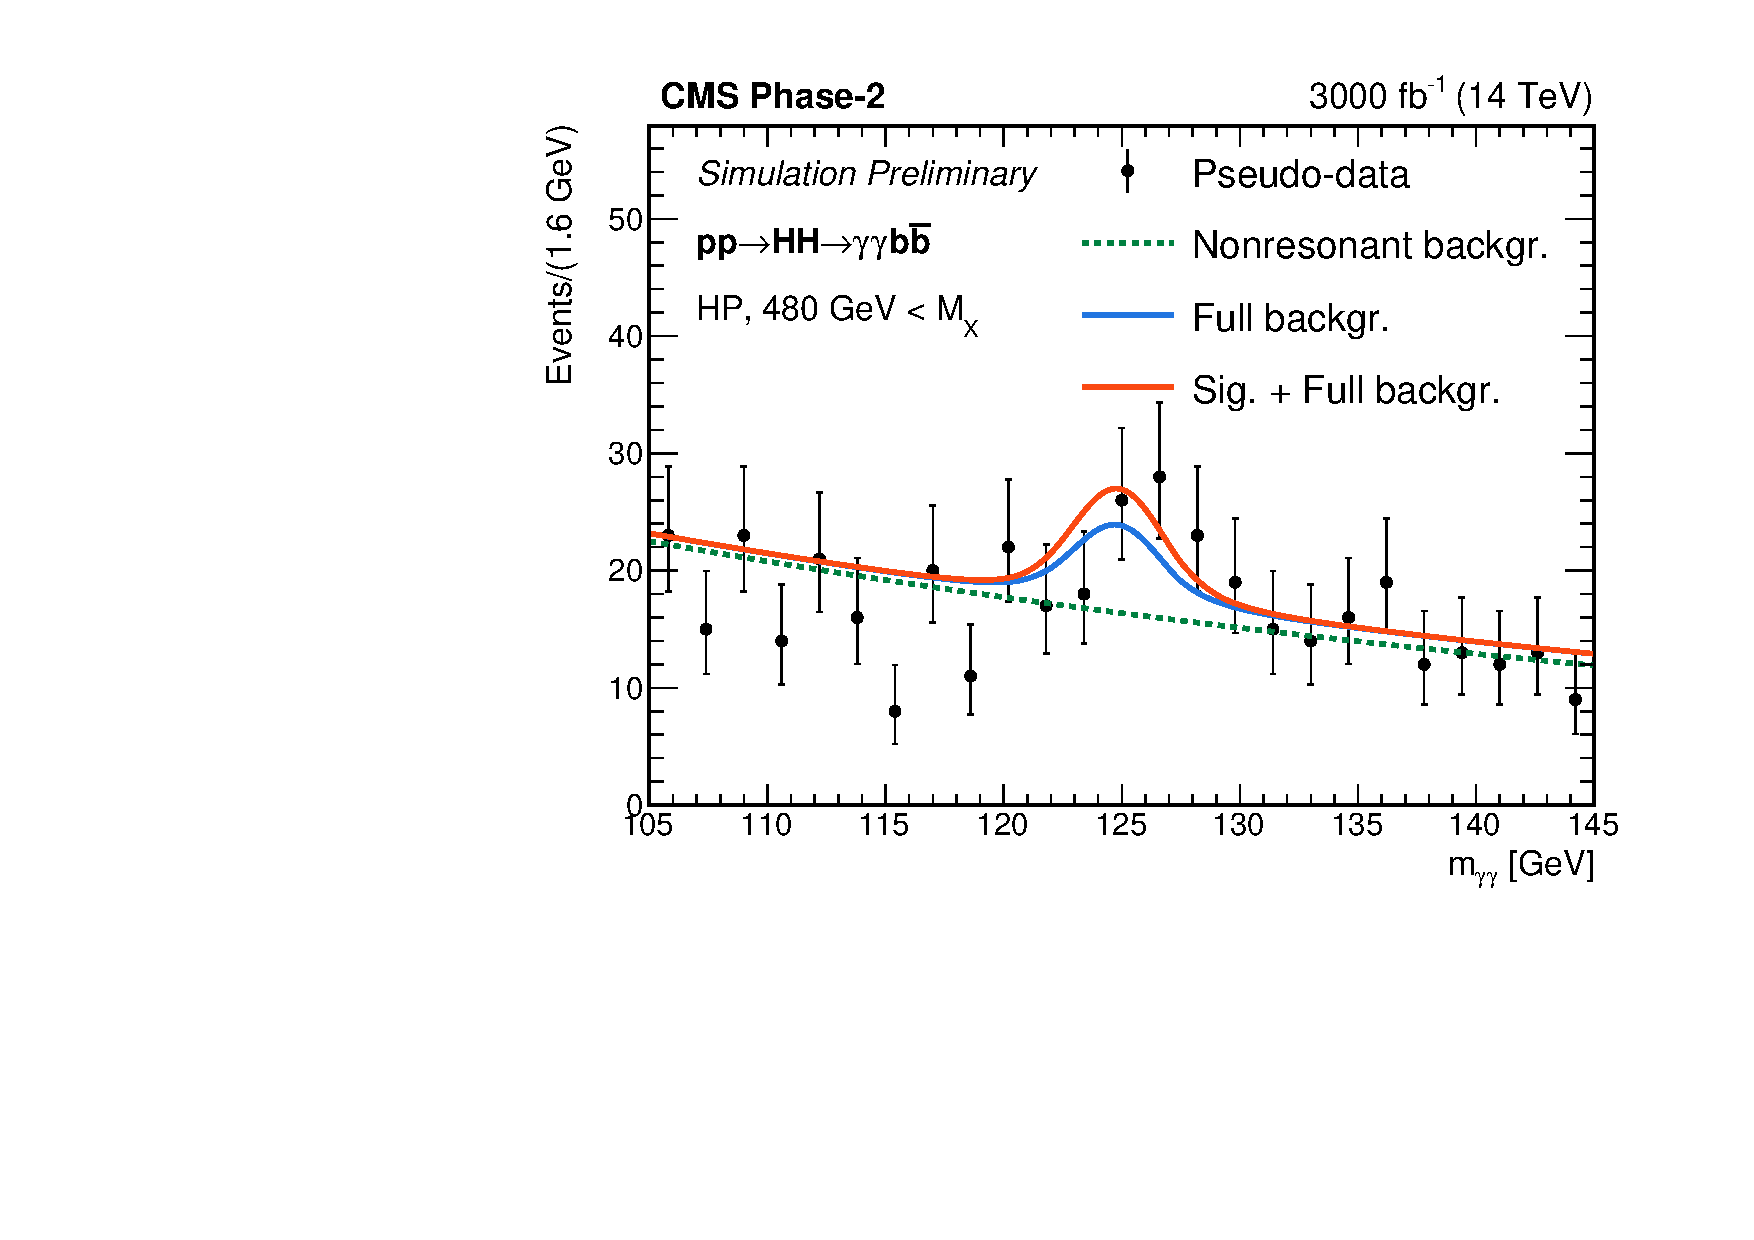
\includegraphics[width=0.495\textwidth]{\main/section3/plots/CMS/Cat4_mgg_poiss.pdf}
    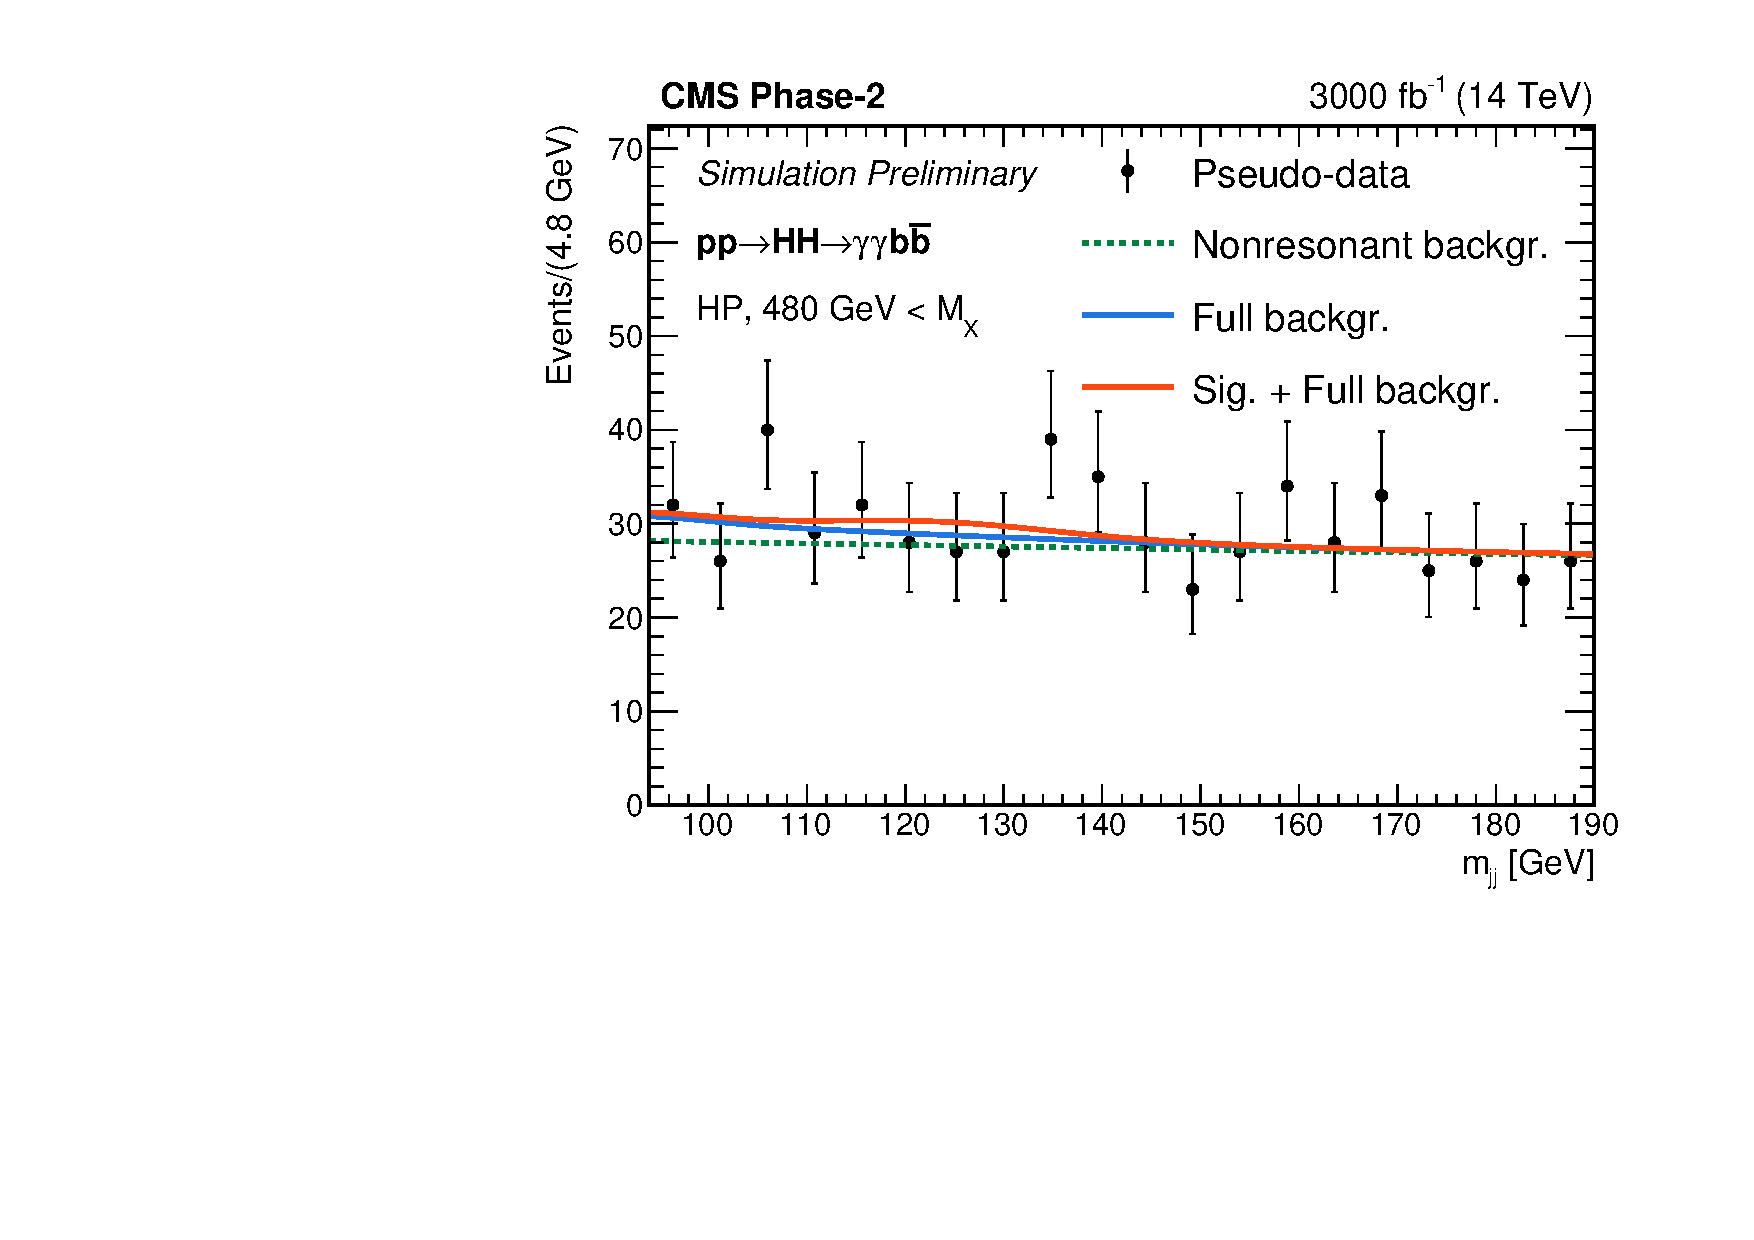
\includegraphics[width=0.495\textwidth]{\main/section3/plots/CMS/Cat4_mjj_poiss.pdf}
\caption{Expected distribution of events in the photon (left column) and jet (right column) pair invariant mass for the high mass and high purity event category. The full circles denote pseudo-data obtained from the expected events yields for the sum of the signal and background processes for $3000\fbinv$.} 
\label{sec3:CMSHH:fig:bbgg_events} 
\end{figure}

\paragraph{The $HH \rightarrow \bbWW \to \PQb\PQb\ell\nu\ell\nu$ channel}

We consider here \HH final states containing two \PQb jets  and two neutrinos and two leptons, either electrons or muons.
The decay channels involved are thus $\PH\to\bb$ in association with either a $\PH\to\PZ(\ell\ell)\PZ(\nu\nu)$ or a $\PH \to \PW(\ell\nu)\PW(\ell\nu)$ decay.
While the analysis described in the following is optimised for $\HH\to\bbWW$ decays, that provide the largest branching fraction, the contribution of Higgs boson decays to both $\PW\PW$ and $\PZ\PZ$, globally denoted as $\text{VV}$, is considered.
Decays of the $\text{VV}$ system to tau leptons subsequently decaying to electrons or muons with the associated neutrinos are also considered in the simulated signal samples.
The corresponding branching fraction for the $\text{VV}\to\ell\nu_\ell\ell\nu_\ell$ decay is 1.73~\%.

The dominant and sub-dominant background processes are
the $\ttbar$ production in its fully leptonic decay mode, and
Drell-Yan production of lepton pairs in association with jets.
As both are irreducible background processes, \ie they result in the same final state as the signal, the kinematic properties of the signal and background events are used and combined in an artificial Neural Network (NN) discriminant to enhance the sensitivity.

Events are required to contain two isolated leptons of opposite electric charge, with an invariant mass $m_{\ell\ell} > 12
\UGeV$ to suppress leptonia resonances and $m_{\PZ} - m_{\ell\ell} > 15\GeV$ to suppress Drell-Yan lepton pair production.
The $\PH\to\PQb\PQb$ decay is reconstructed by requiring the presence of two b-tagged jets in the event with $\pt > 20$~\UGeV and $| \eta | < 2.8$, separated from the selected leptons by a distance of $\Delta \text{R} = \sqrt{\Delta \phi^2 + \Delta \eta^2} > 0.3$.

% Events are required to contain two leptons of opposite electric charge
% ($\Pe^{+}\Pe^{-}, \mu^{+}\mu^{-}, \Pe^{\pm}\mu^{\mp}$), and with \pt greater than 25~GeV and 15~GeV for
% $\Pe\Pe$ events, 20~GeV and 10~GeV for $\mu\mu$ events, 25~GeV and 15~GeV for
% $\mu\Pe$ events, 25~GeV and 10~GeV for $\Pe\mu$ events, for the higher and lower \pt lepton,
% respectively. Electrons and muons in the pseudo-rapidity range
% $| \eta | < 2.8$ are considered, except the $ 1.444 < | \eta | < 1.5666$ being rejected for electrons.
% A dilepton mass requirement of $m_{\ell\ell} > 12$~GeV is applied to all flavour combinations in
% order to suppress lepton onia resonances.


% Jets are required to have
% $\pt > 20$~GeV, $| \eta | < 2.8$, and be separated from identified leptons
% by a distance of $\Delta \text{R} = \sqrt{\Delta \phi^2 + \Delta \eta^2} > 0.3$.
% The magnitude of the negative vector sum of all PF candidates is referred
% to as $\ptmiss$. 
% Selected jets must also satisfy the medium working point of the b tagging algorithm.

% A neural network (NN) discriminant is used to improve the signal-to-background
% separation.
The NN discriminant utilises information related
to object kinematics.
The variables provided as input to the NN exploit the presence of two Higgs  bosons decaying into two b-jets on the one hand, and two leptons and two neutrinos on the other hand, 
which results in different kinematics for the di-lepton and di-jet systems between signal and 
background processes.
The set of variables used as input is:$ m_{\ell\ell}$, $m_\text{jj}$,
$\Delta R_{\ell\ell}$, $\Delta R_{\text{j}\text{j}}$, $\Delta \phi_{\ell\ell, \text{j}\text{j}}$, defined as 
the $\Delta \phi$ between the di-jet and the di-lepton systems, $\pt^{\ell\ell}$, $\pt^{\text{j}\text{j}}$,
min$\left(\Delta R_{\text{j}, \ell}\right)$, and $\mathrm{M}_\mathrm{T}$, defined as
$\mathrm{M}_\mathrm{T} = \sqrt{2 \pt^{\ell\ell} \ptmiss (1 - \cos(\Delta \phi(\ell\ell, \ptmiss)))}$.

The output of the NN is used as the discriminant variable in the three decay channels studied, and its distribution is reported in Fig.~\ref{sec3:CMSHH:fig:bbWW_events}.

\begin{figure}[!htb]
  \begin{center}
    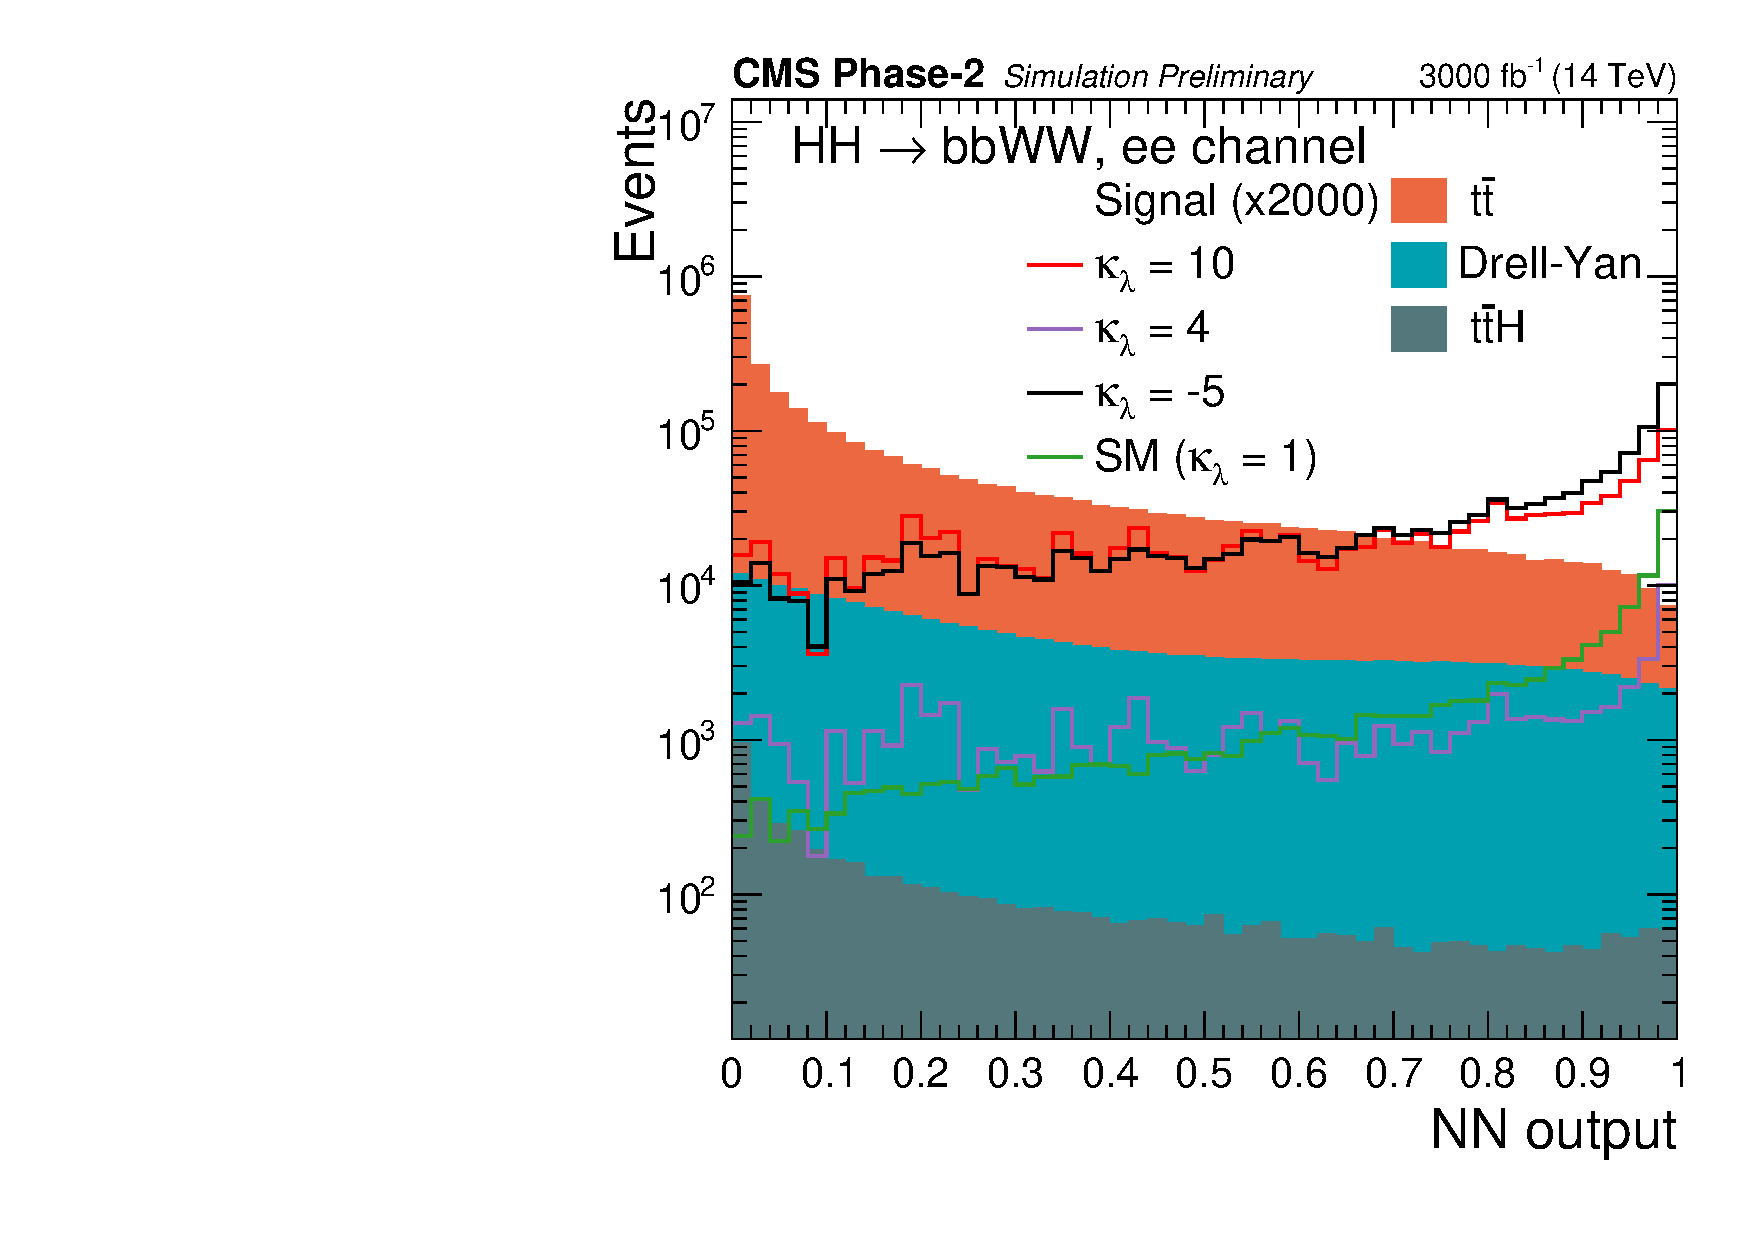
\includegraphics[width=0.32\textwidth]{\main/section3/plots/CMS//NN_nonresonant_point_1p00_1p00_ElEl_hh_llmetjj_HWWleptons_btagM_cmva_mll_cut_rebin_final_logy.pdf}
    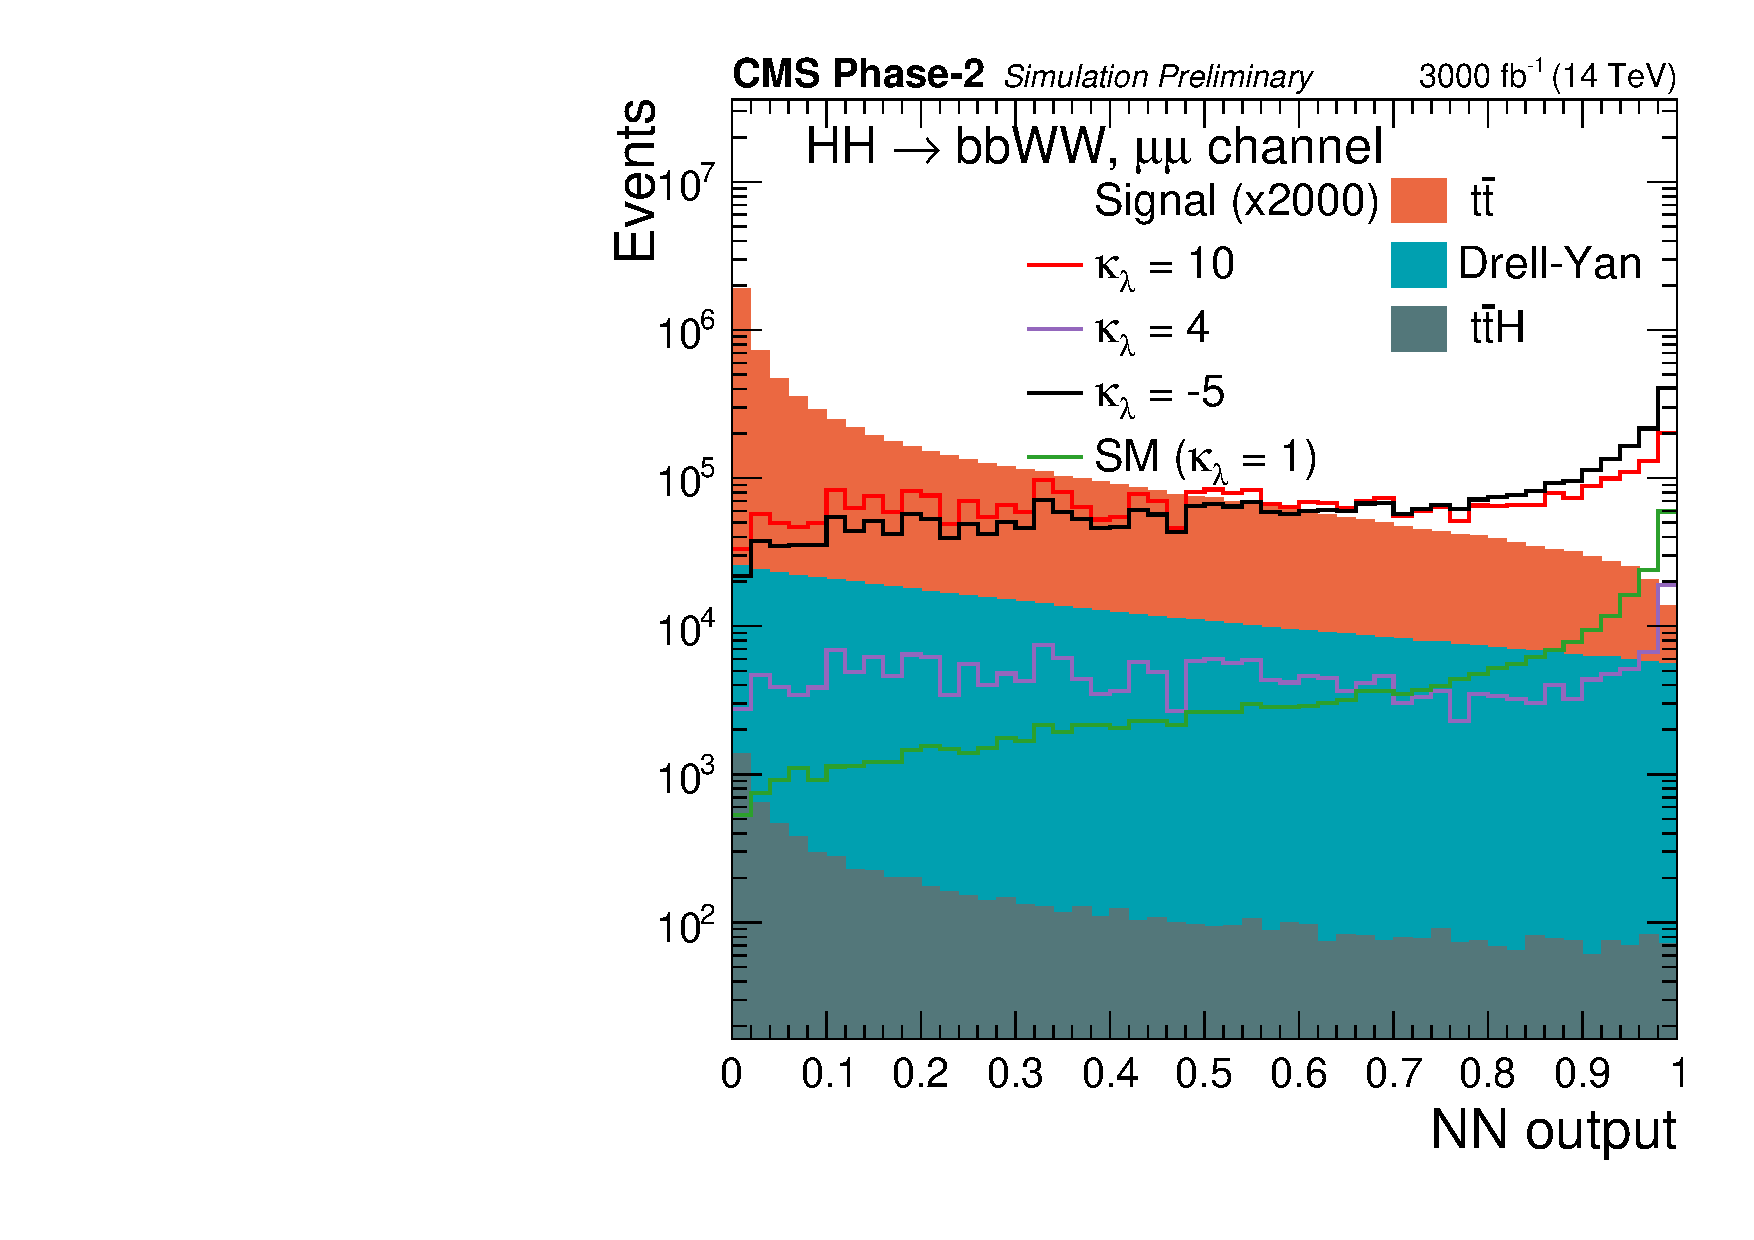
\includegraphics[width=0.32\textwidth]{\main/section3/plots/CMS//NN_nonresonant_point_1p00_1p00_MuMu_hh_llmetjj_HWWleptons_btagM_cmva_mll_cut_rebin_final_logy.pdf}
    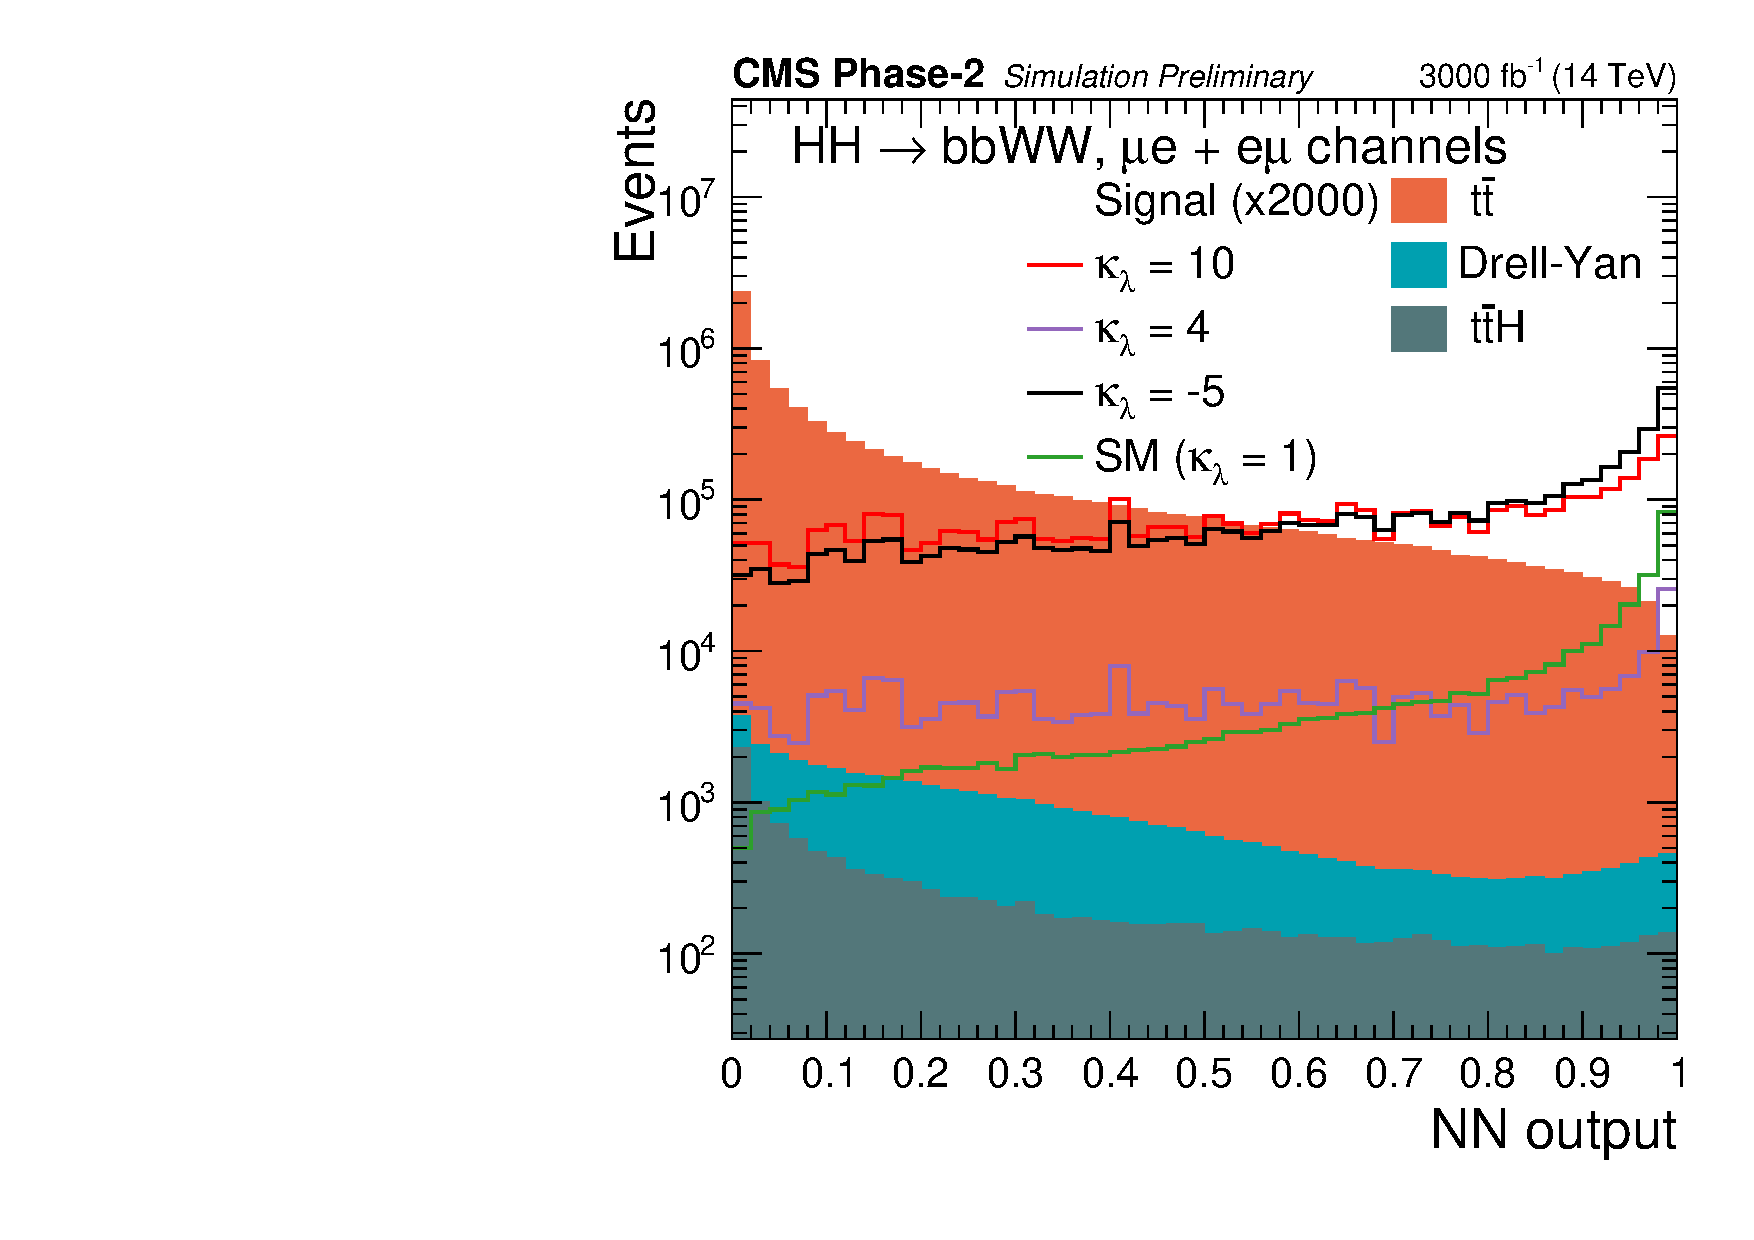
\includegraphics[width=0.32\textwidth]{\main/section3/plots/CMS//NN_nonresonant_point_1p00_1p00_MuEl_hh_llmetjj_HWWleptons_btagM_cmva_mll_cut_rebin_final_logy.pdf}
    \caption{
      The output of the $\bbWW$ NN after the selections, evaluated in the
      $\Pe^{+}\Pe^{-}$~(left) , $\mu^{+}\mu^{-}$~(middle),
      $\Pe^{\pm}\mu^{\mp}$~(right) channels.
    }
    \label{sec3:CMSHH:fig:bbWW_events}
  \end{center}
\end{figure}


\paragraph{The $\HH\to\bbZZ\to \PQb\PQb 4\ell$ channel}

The \HH searches at the LHC have so far focused on final states with a sizeable branching ratio because of the small cross section of this process.
The HL-LHC will open the possibility to study rare but clean decay channels thanks to the large dataset available.
The $\bbZZ(4\ell)$ channel, that is investigated in this work, benefits from the clean four lepton signature to clearly identify signal events in the busy pileup environment of the HL-LHC.

Events are required to have at least four identified and isolated (isolation < 0.7) muons (electrons) with $\pt > 5(7)\GeV$ and $|\eta|< 2.8$. 
The two $\PZ$ boson candidates are formed from pairs of opposite-charge leptons
The $\PZ$ candidate with the invariant mass closest to the nominal Z mass is denoted as $\PZ_1$, while the other one is labelled as $\PZ_2$.
$\PZ$ candidates are required to have an invariant mass in the range [40, 120] \UGeV ($\PZ_1$) and [12, 120] \UGeV ($\PZ_2$), respectively.
%At least one lepton is required to have $p_T >$ > 20 GeV and a second is required to have $p_T >$ > 10 GeV.
%On figure~\ref{fig:CMS_HH4l} we show the resolution of the reconstructed $H \rightarrow ZZ \rightarrow 4l$ after baseline selections.
The four leptons invariant mass is requested to be in the range [120,130] \UGeV.
At least two (but not more than three) b-tagged jets are also required to be  present  and have an invariant mass.
The jet pair is required to have an invariant mass in the range [80, 160] \UGeV and an angular distance between the 2 jets between 0.5 and 2.3.
The number of events thus selected are used to look for the presence of a signal on top of the background processes, mostly constituted of single Higgs boson production in the $4\ell$ final state.
The distribution of the four lepton invariant mass is shown in  Fig,~\ref{sec3:CMSHH:fig:bbZZ_events}.


\begin{figure}[!htb]
  \begin{center}
    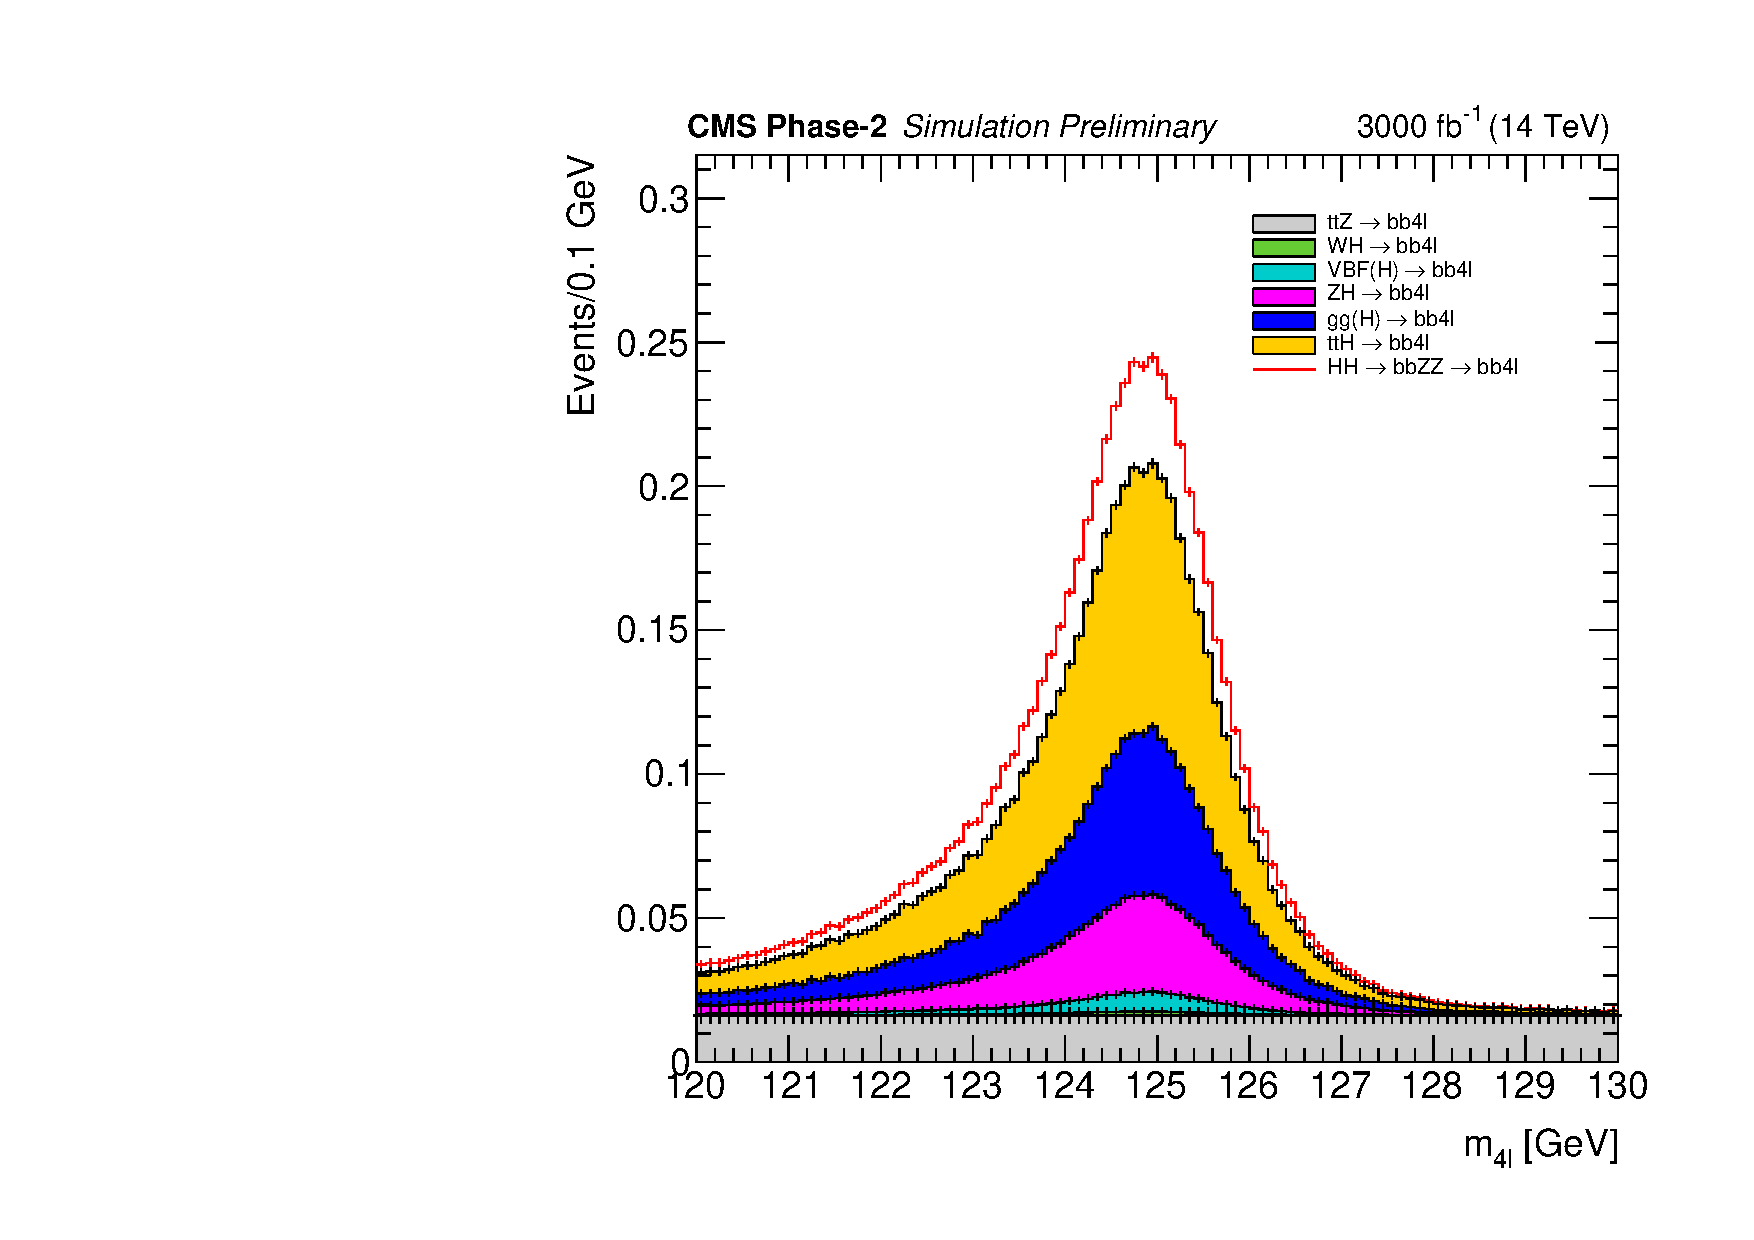
\includegraphics[width=0.49\textwidth]{\main/section3/plots/CMS/Mass_4l.pdf}
    \caption{Invariant mass distribution of the four leptons selected at the end of the analysis for the $\PQb\PQb 4\ell$ final state.}
    \label{sec3:CMSHH:fig:bbZZ_events}
  \end{center}
\end{figure}


\paragraph{Combined results}

The five decay channels are combined statistically assuming the SM Higgs boson branching fractions.
Assuming the presence of a signal with the properties predicted by the SM, its total expected  significance is $2.6\sigma$.
If instead the background only hypothesis is assumed, an expected upper limit on the SM \HH signal cross section can be set to 0.77 times the SM prediction.
The contributions from the five decay channels and the combined expected sensitivities are reported in Tab.~\ref{sec3:cMSHH:tab:comb}.

\begin{table}[htp]
\centering
\caption{Upper limit at the 95\% confidence level, significance, projected measurement at 68\% confidence level of the Higgs boson self coupling $\lambdahhh$ for the five channels studied and their combination. Systematic and statistical uncertainties are considered.}
\label{sec3:cMSHH:tab:comb}
\begin{tabular}{l c c c c}
    \toprule
    \multirow{2}{*}{Channel} & \multicolumn{2}{c}{Significance} & \multicolumn{2}{c}{95\% CL limit on $\sigma_{\HH}/\sigma_{\HH}^\text{SM}$} \\
    % \cmidrule(lr){2-3}
    % \cmidrule(lr){4-5}
                             & Stat. + syst.  & Stat. only &  Stat. + syst. & Stat. only \\
    \cmidrule(lr){2-3}
    \cmidrule(lr){4-5}
    % \midrule
    \bbbb                     & 0.95 & 1.2  & 2.1  & 1.6 \\
    \bbtt                     & 1.4  & 1.6  & 1.4  & 1.3 \\
    $\bbWW(\ell\nu\ell\nu)$   & 0.56 & 0.59 & 3.5  & 3.3 \\
    \bbgg                     & 1.8  & 1.8  & 1.1  & 1.1 \\
    $\bbZZ(\ell\ell\ell\ell)$ & 0.37 & 0.37 & 6.6  & 6.5\\
    \midrule
    Combination               & 2.6  & 2.8  & 0.77 & 0.71 \\
    \bottomrule
\end{tabular}
\end{table} 

% In case a \HH signal is found at the HL-LHC with a signifance compatible with the one detailed above, the observation can be used to constrain the trilinear Higgs boson self-coupling \lambdahhh.
% Assuming that no \HH signal exists, the expected dependence of the likelihood function on $k_\lambda = \lambdahhh / \lambdahhh^\text{SM}$ is shown in Fig.~\ref{}\fixme{placeholder}.
% The reader can observe the presence of two minims, one corresponding to $k_\lambda = 1$ and the second at larger $k_\lambda$ values.
% The latter is a consequence of the dependence of the total \HH production cross section as a function of $k_\lambda$, that is symmetric around $k_\lambda \approx 2.5$.
% The degeneracy is reduced once differential information on the $m_{\HH}$ distribution are used, as done with the mass categorisation used in the $\bbgg$ search.
% The projected measurement of the Higgs boson self-coupling corresponds to [xxx, yyy] at 68\% CL and to [xxx, yyy] at 95\% CL.

% Similarly, assuming the absence of any \HH signal, it is possible to exclude at the 95\% CL values of $k_\lambda$ below xxx or above yyy, as shown in Fig.~\ref{}\fixme{placeholder}.
% In particular, the enhanced \HH cross section for $k_\lambda = 0$ will allow to establish the existence of a Higgs boson self coupling at the HL-LHC, as this hypothesis will be excluded at the 95\% CL.

Prospects for the measurement of the Higgs boson self coupling are also studied.
Under the assumption that no \HH signal exists, 95\% CL upper limits on the SM \HH production cross section are derived as a function $\kappa_\lambda = \lambdahhh/\lambdahhh^\text{SM}$, where $\lambdahhh^\text{SM}$ denotes the SM prediction. 
The result is illustrated in Fig.~\ref{sec3:CMSHH:fig:comb_plots}.
A variation of the excluded cross section, directly related to changes in the \HH kinematic properties, can be observed as a function of $\kappa_\lambda$.

% \begin{figure}[htbH]
%   \centering
%     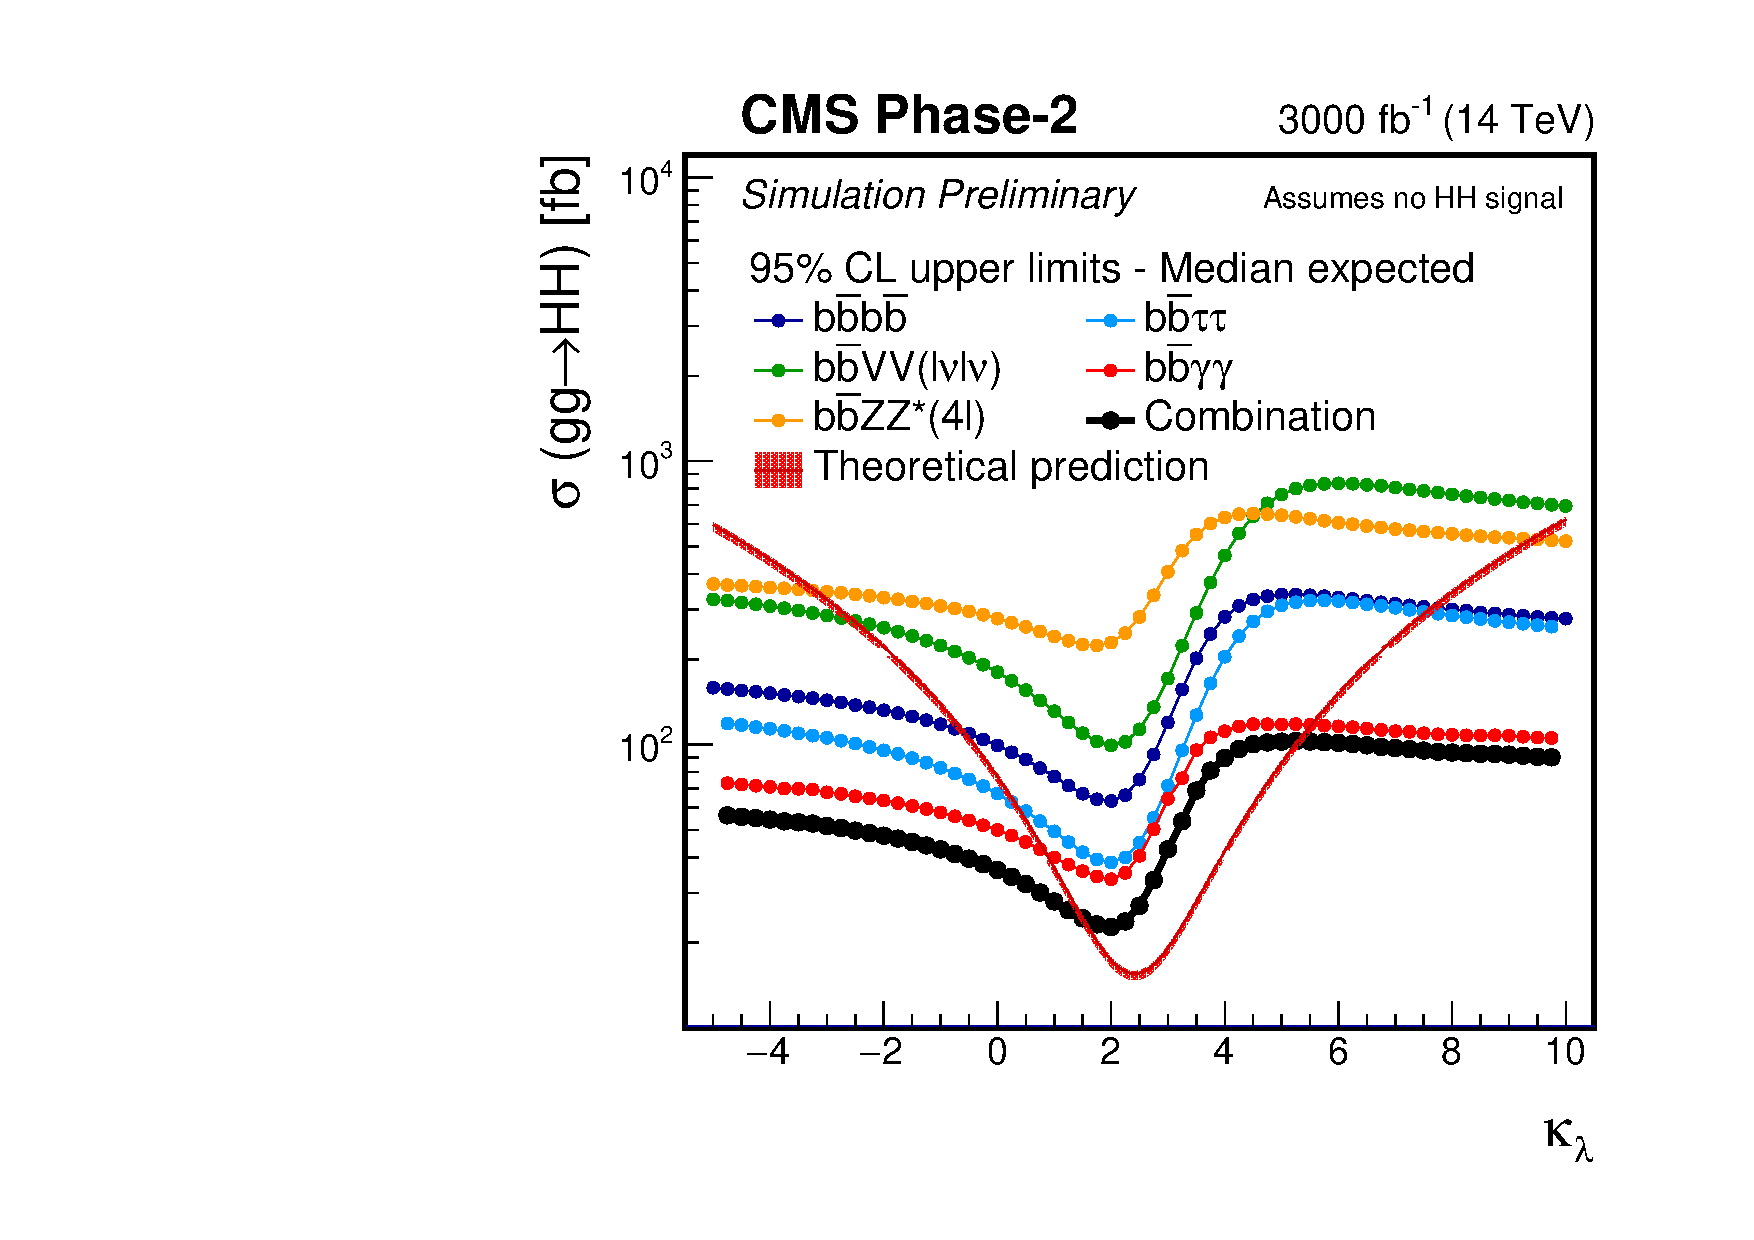
\includegraphics[width=0.6\textwidth]{\main/section3/plots/CMS/limit_comparison.pdf}
%     \caption{Upper limit at the 95\% CL on the \HH production cross section as a function of $\kapl = \lambdahhh/\lambdahhh^\text{SM}$ for the five decays channels investigated and their combination. The red band indicated the theoretical production cross section.}
%     \label{fig:comb:limit_scan}
% \end{figure}

Assuming instead that a \HH signal exists with the properties predicted by the SM, prospects for the measurement of the \lambdahhh are derived.
The scan of the likelihood as a function of the \kapl coupling is shown in Fig.~\ref{sec3:CMSHH:fig:comb_plots}.
The projected confidence interval on this coupling corresponds to $[0.35, 1.9]$ at the 68\% CL and to $[-0.18, 3.6]$ at the 95\% CL.
The peculiar likelihood function structure, characterised by two local minimums, is related to the dependence of the total cross section and \HH kinematic properties on $\kapl$, while the relative height of the two minimums depends to the capability of the analyses to access differential $m_{\HH}$ information.
The degeneracy of the second minimum is largely removed thanks to the $\bbgg$ analysis and its $m_{\HH}$ categorisation.


% \begin{figure}[htbH]
%   \centering
%     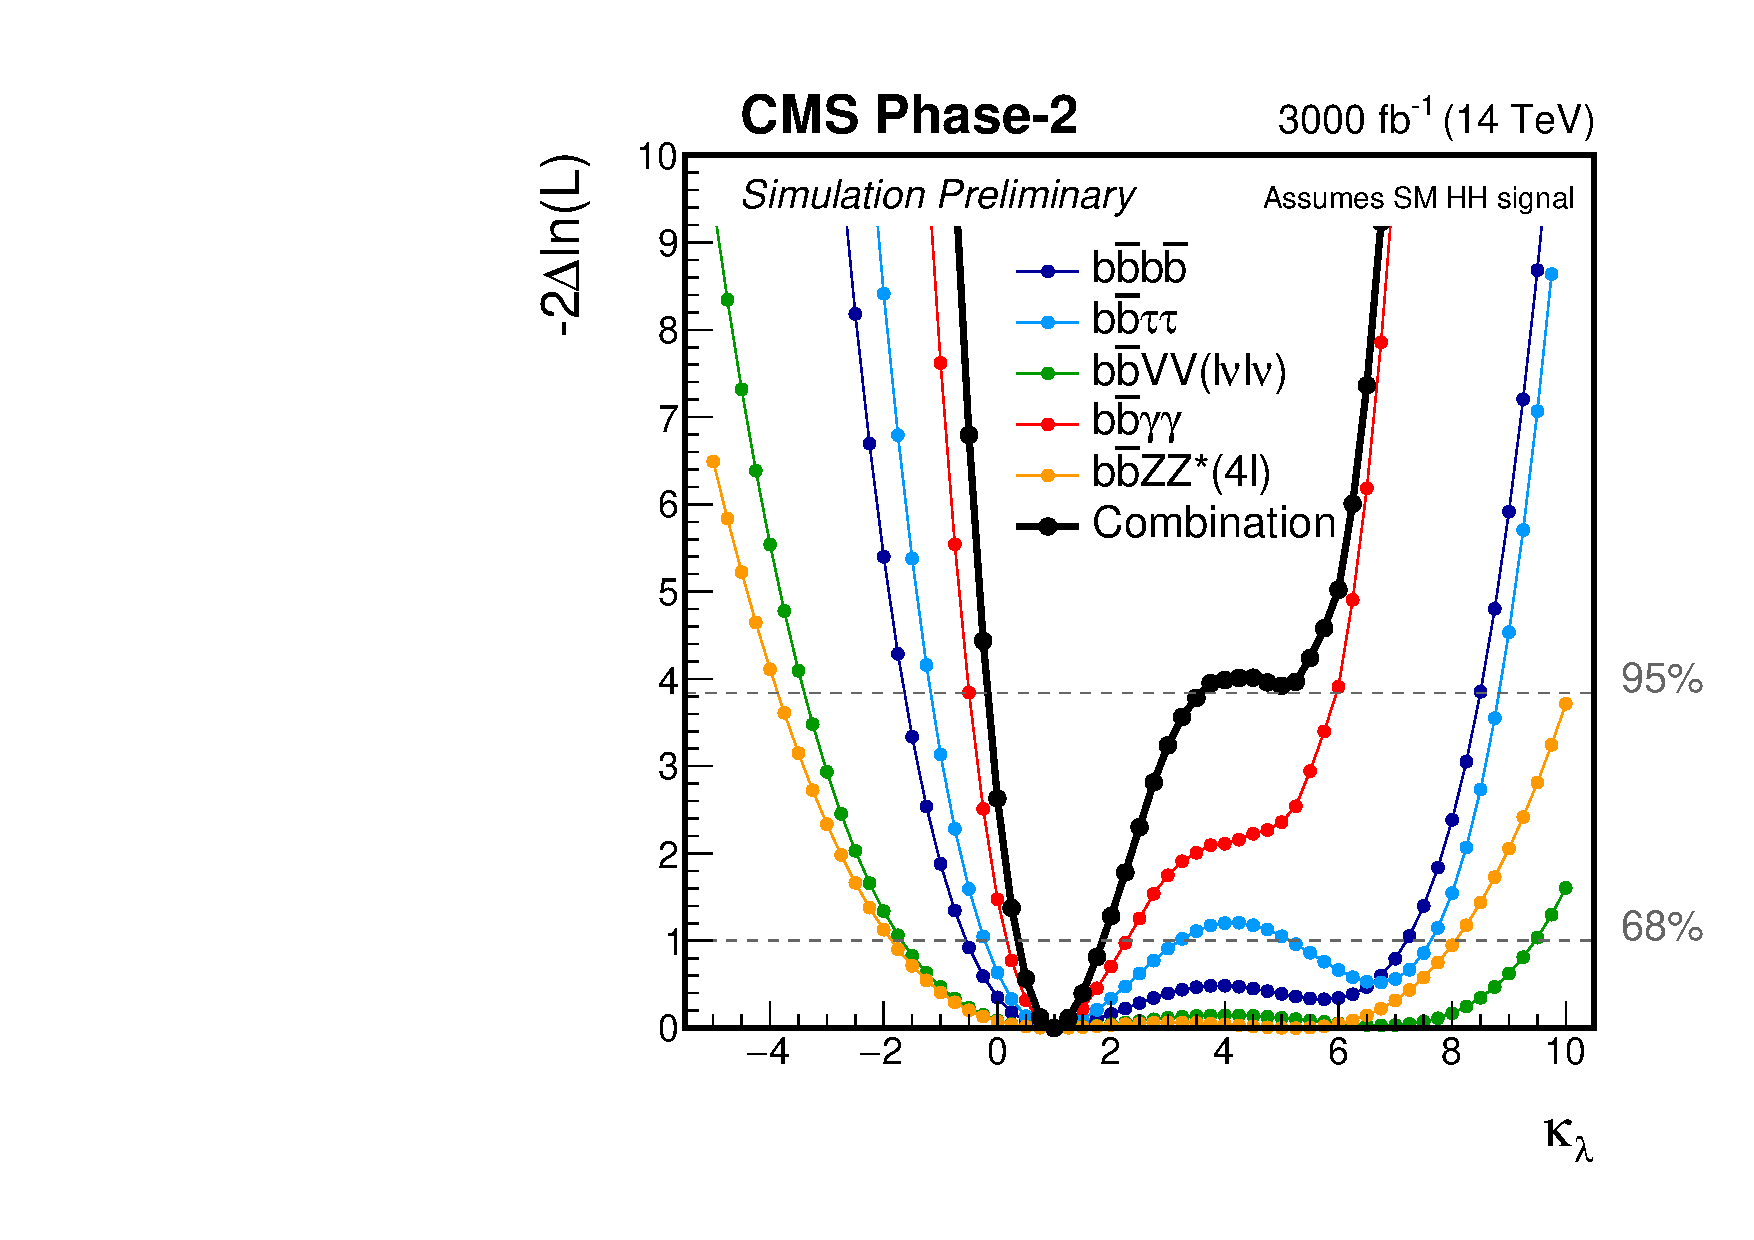
\includegraphics[width=0.6\textwidth]{\main/section3/plots/CMS/likelihood_comparison.pdf}
%     \caption{Expected likelihood scan as a function of $\kappa_\lambda = \lambdahhh/\lambdahhh^\text{SM}$. The functions are shown separately for the five decay channels studied and for their combination.}
%     \label{fig:comb:likelihood_scan}
% \end{figure}

\begin{figure}[htb]
  \centering
   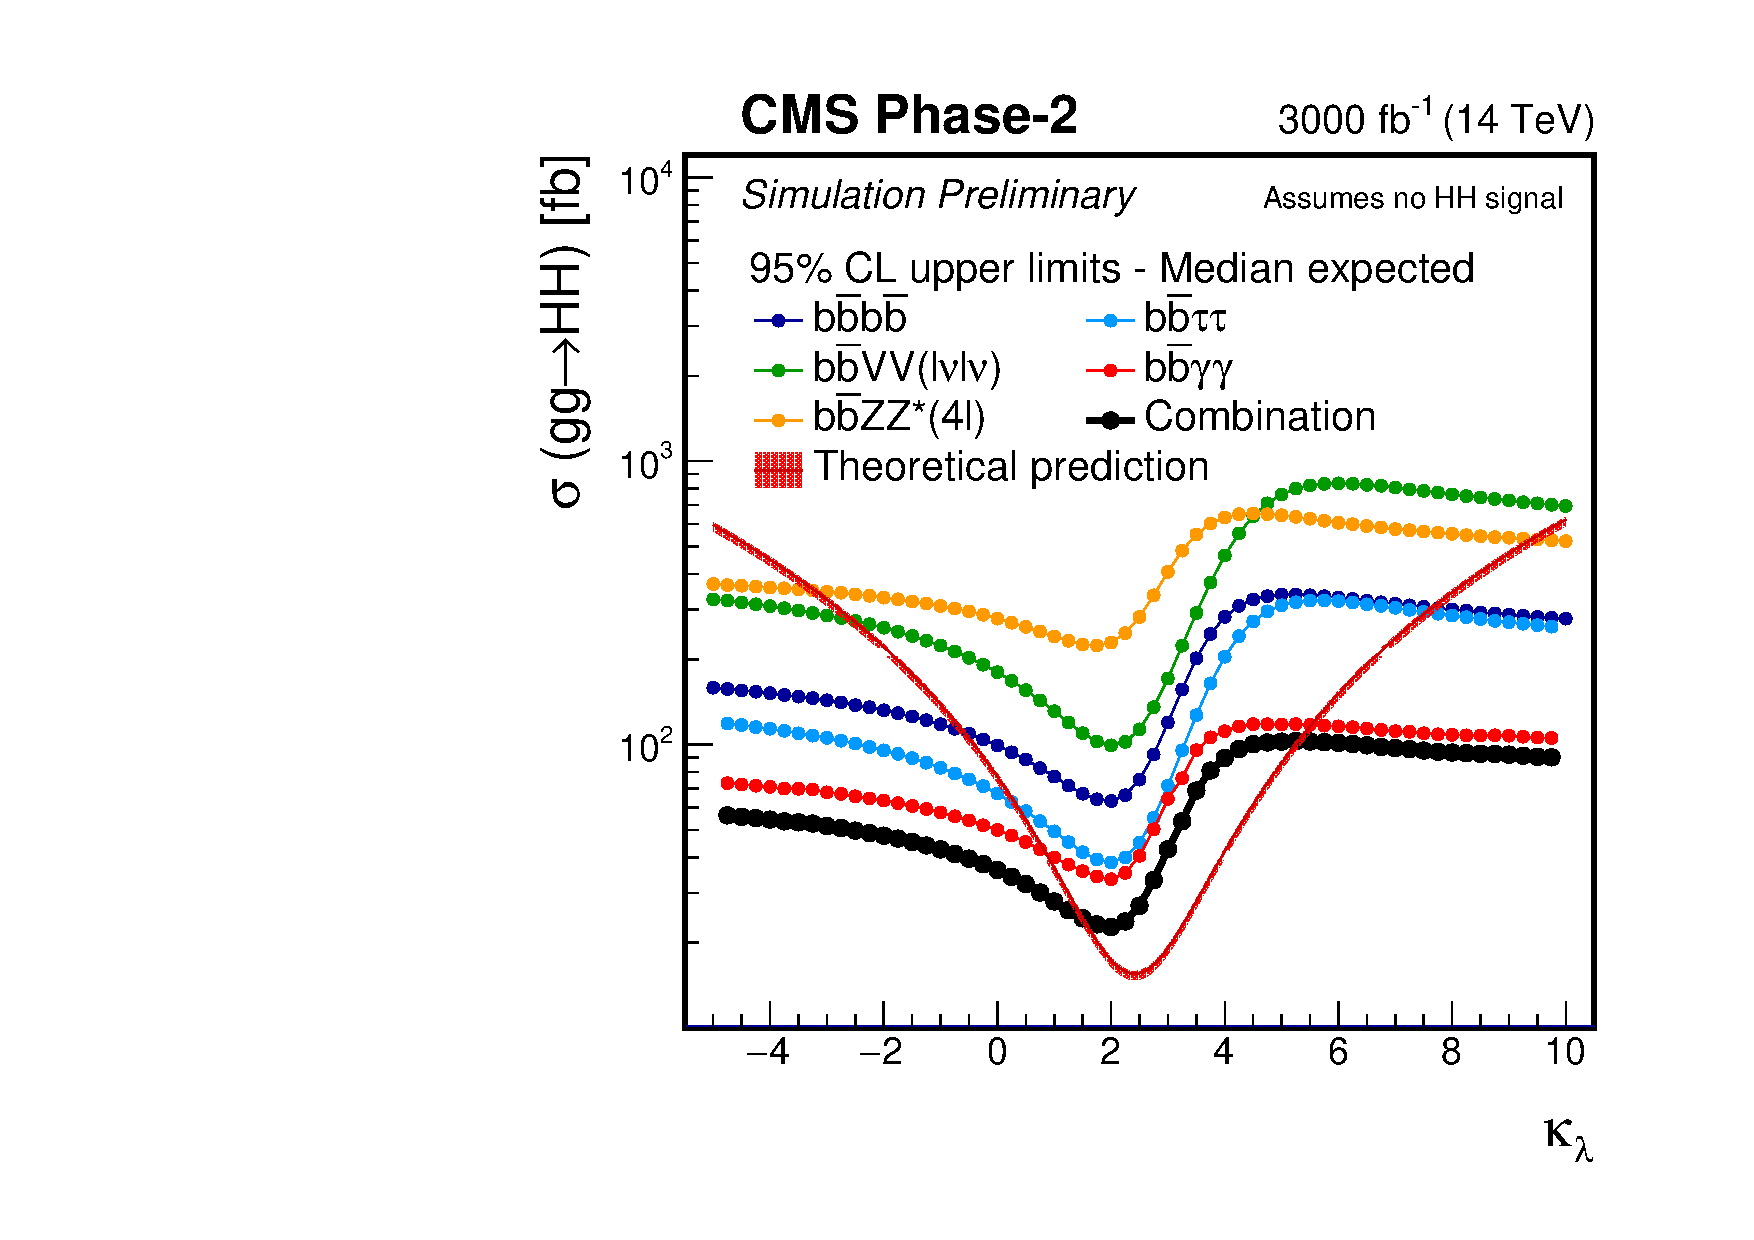
\includegraphics[width=0.48\textwidth]{\main/section3/plots/CMS/limit_comparison.pdf}
    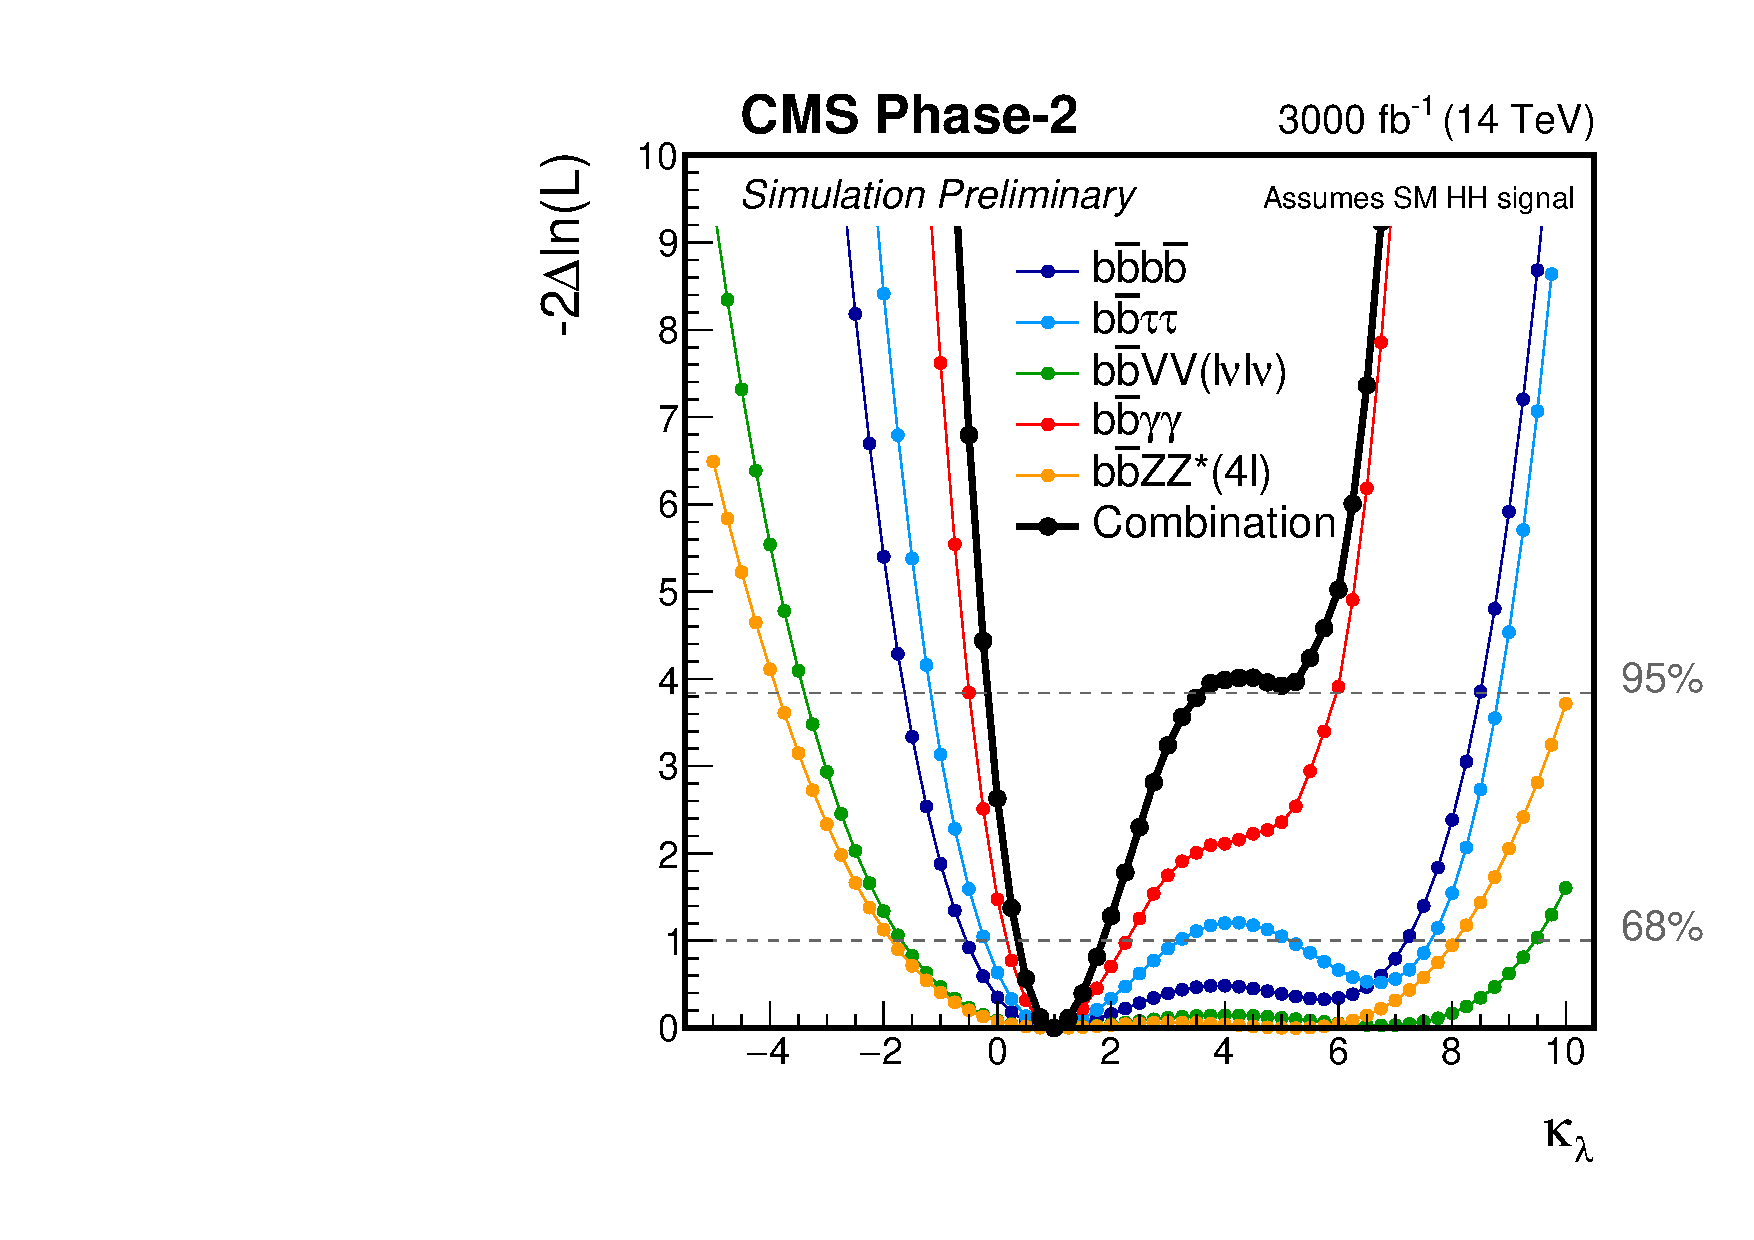
\includegraphics[width=0.48\textwidth]{\main/section3/plots/CMS/likelihood_comparison.pdf}
    \caption{Left: upper limit at the 95\% CL on the \HH production cross section as a function of $\kapl = \lambdahhh/\lambdahhh^\text{SM}$. The red band indicated the theoretical production cross section. Right: expected likelihood scan as a function of $\kappa_\lambda = \lambdahhh/\lambdahhh^\text{SM}$. In both figures the results are shown separately for the five decay channels studied and for their combination.}
    \label{sec3:CMSHH:fig:comb_plots}
\end{figure}
